\chapter{MODELAGEM FÍSICA E METODOLOGIA}
\label{chapter:metodologia}

Para validar a teoria matemática exposta no Capítulo \ref{chapter:revisao}, desenvolveu-se um protótipo físico articulado. Este capítulo descreve a construção mecânica do mecanismo robótico, apresentando a lista de insumos utilizados, as ferramentas aplicadas e a extração dos parâmetros geométricos de cada membro que compõe o sistema.

\section{Construção do Protótipo}
\label{sec:construcao}

A concepção física do mecanismo robótico foi inspirada em tutoriais e modelos educacionais de mecanismos articulados disponíveis no YouTube. O projeto foi adaptado para atender aos requisitos rigorosos de análise cinemática e cinética exigidos na disciplina de Dinâmica, garantindo que o movimento real do sistema pudesse ser descrito pelas equações vetoriais de Newton-Euler \cite{hibbeler2016}.

O foco da montagem foi a utilização de materiais de baixo custo e fácil manipulação, garantindo, ao mesmo tempo, a rigidez estrutural necessária para suportar os esforços gerados pelo acionamento do motor DC com redução.

A \ref{tab:quant_materiais} detalha o inventário de todos os componentes, insumos e ferramentas empregados na fabricação e montagem do protótipo robótico.

\begin{table}[H]
\centering
\caption{\label{tab:quant_materiais}- Relação quantitativa de materiais, insumos e ferramentas.}
\vspace*{.1cm}
\begin{tabular}{|l|c|c|}
\hline
\textbf{Item / Descrição} & \textbf{Categoria} & \textbf{Quantidade} \\
\hline
Palito de Picolé & Insumo (Estrutura) & 10 unidades \\ % Preencha a quantidade
\hline
Palito de Churrasco & Insumo (Eixos) & 03 unidades \\
\hline
Adesivo Instantâneo (Tekbond) & Insumo (Fixação) & 1 frasco \\
\hline
Cola Quente (Bastão) & Insumo (Preenchimento) & 01 unidades \\
\hline
Motor DC com Caixa de Redução & Componente Eletromecânico & 1 unidade \\
\hline
Bateria & Componente Eletromecânico & 1 unidade \\
\hline
Alicate de Corte & Ferramenta & 1 unidade \\
\hline
Micro Retífica & Ferramenta & 1 unidade \\
\hline
Paquímetro (resolução de 0,05 mm) & Instrumento de medição & 1 unidade \\
\hline
Balança de precisão & Instrumento de medição & 1 unidade \\
\hline
\end{tabular}
\end{table}

\subsection{Registro Fotográfico dos Insumos e Ferramentas}

A fim de documentar o processo de fabricação, as figuras a seguir ilustram individualmente cada um dos materiais e ferramentas listados na \ref{tab:quant_materiais}: os dois tipos de palito (\ref{fig:mat_picole} e \ref{fig:mat_churrasco}), o alicate para corte (\ref{fig:ferr_alicate}), a micro retífica para usinagem e furação (\ref{fig:ferr_retifica}) e o paquímetro usado nas medidas dimensionais (\ref{fig:ferr_paquimetro}).

\begin{figure}[H]
\begin{center}
 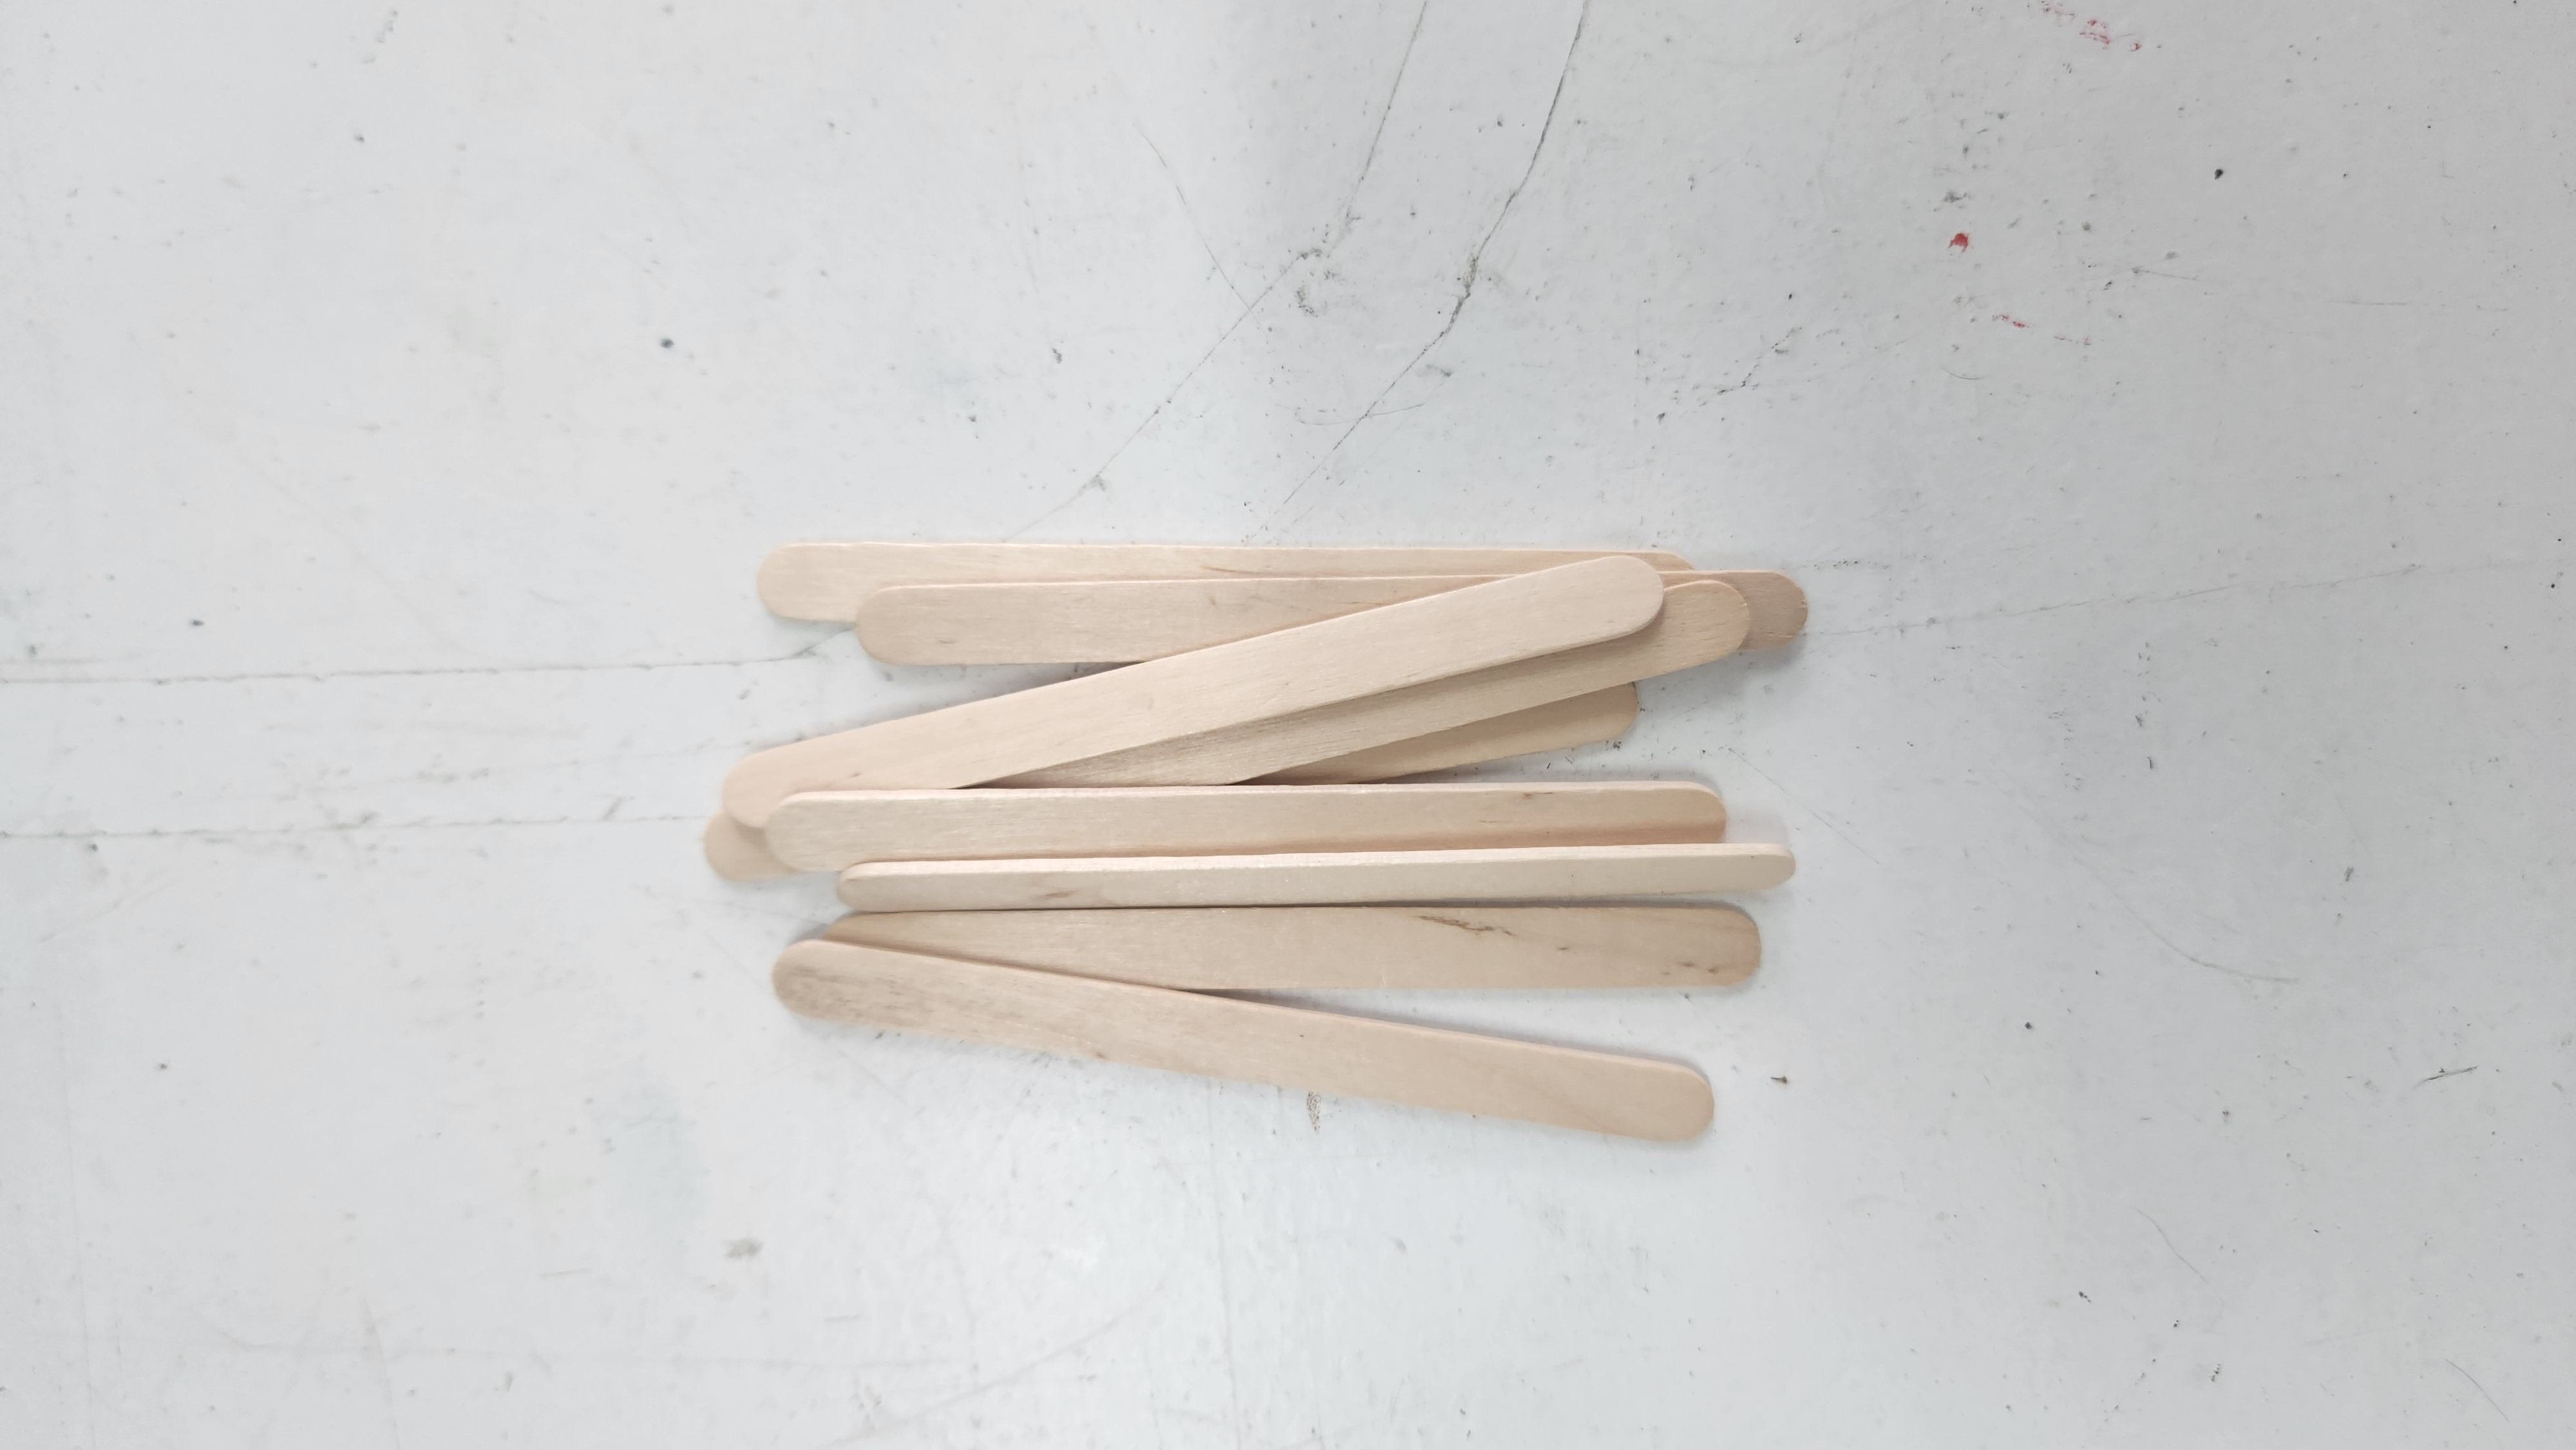
\includegraphics[width=12cm]{foto_palito_picole.jpg}
\caption{\label{fig:mat_picole}- Insumo estrutural: Palitos de picolé.}
\end{center}
\end{figure}

\begin{figure}[H]
\begin{center}
 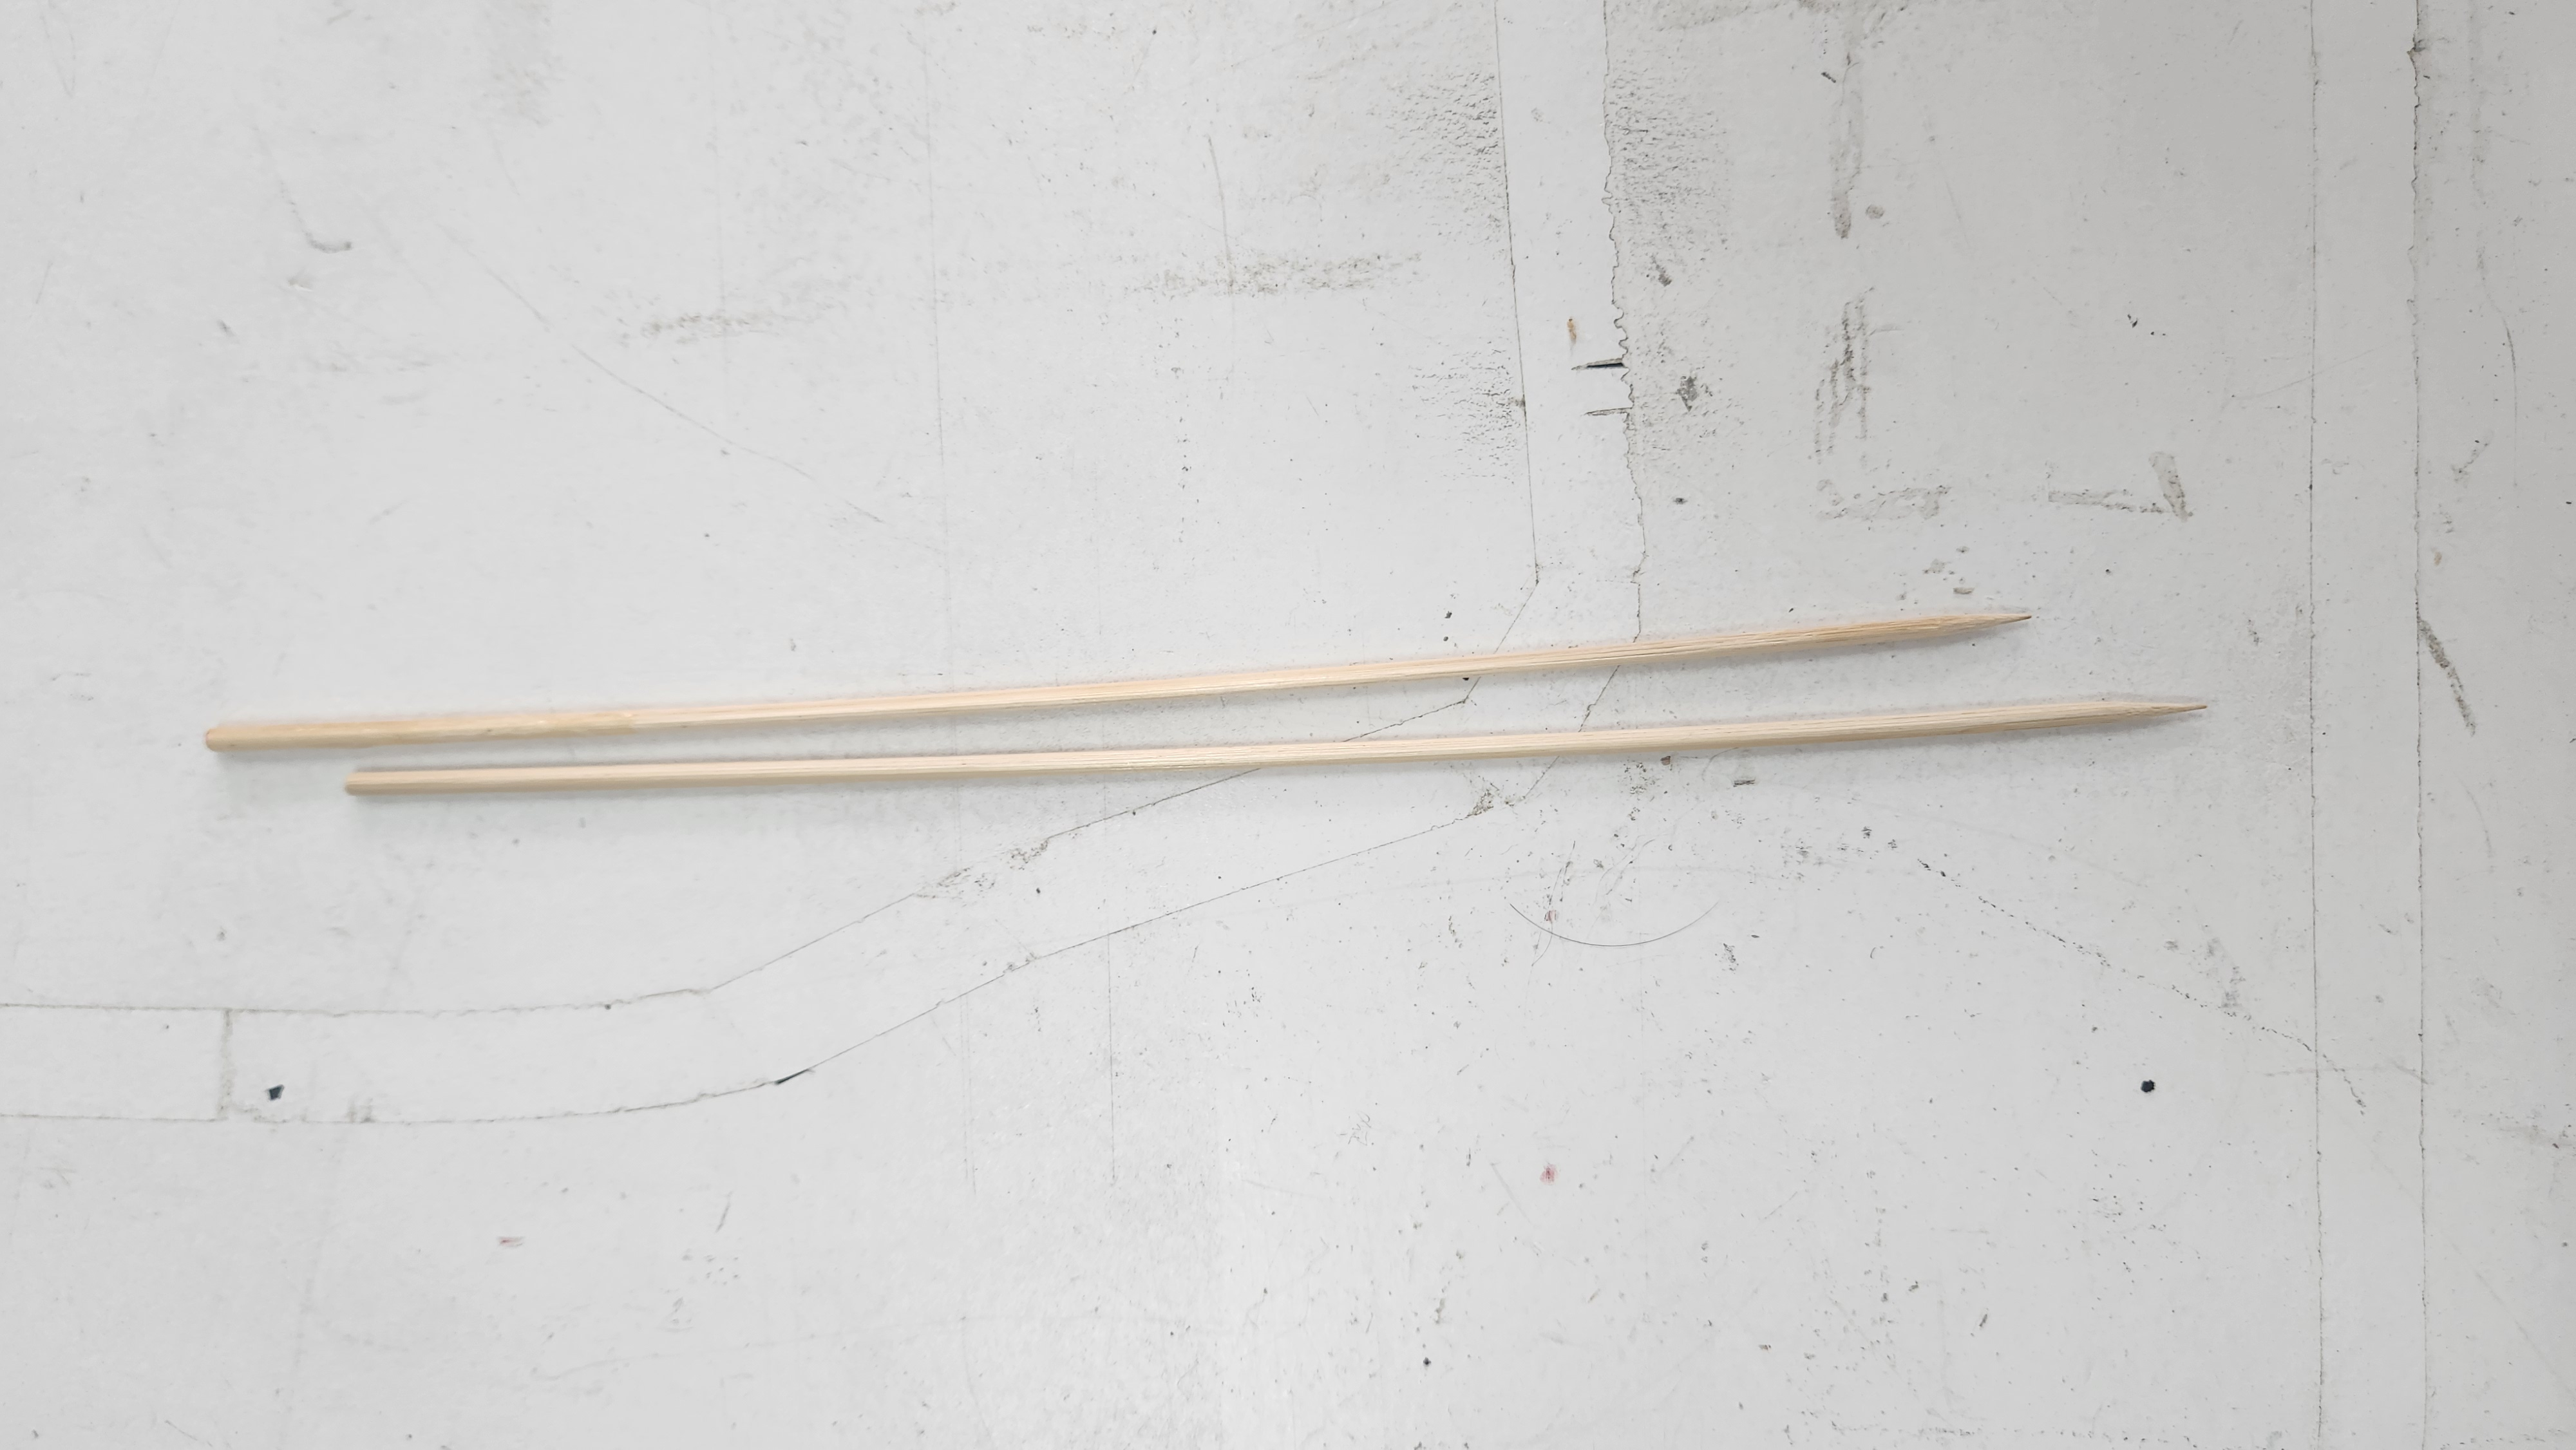
\includegraphics[width=12cm]{foto_palito_churrasco.jpg}
\caption{\label{fig:mat_churrasco}- Insumo para eixos de articulação: Palitos de churrasco.}
\end{center}
\end{figure}



\begin{figure}[H]
\begin{center}
 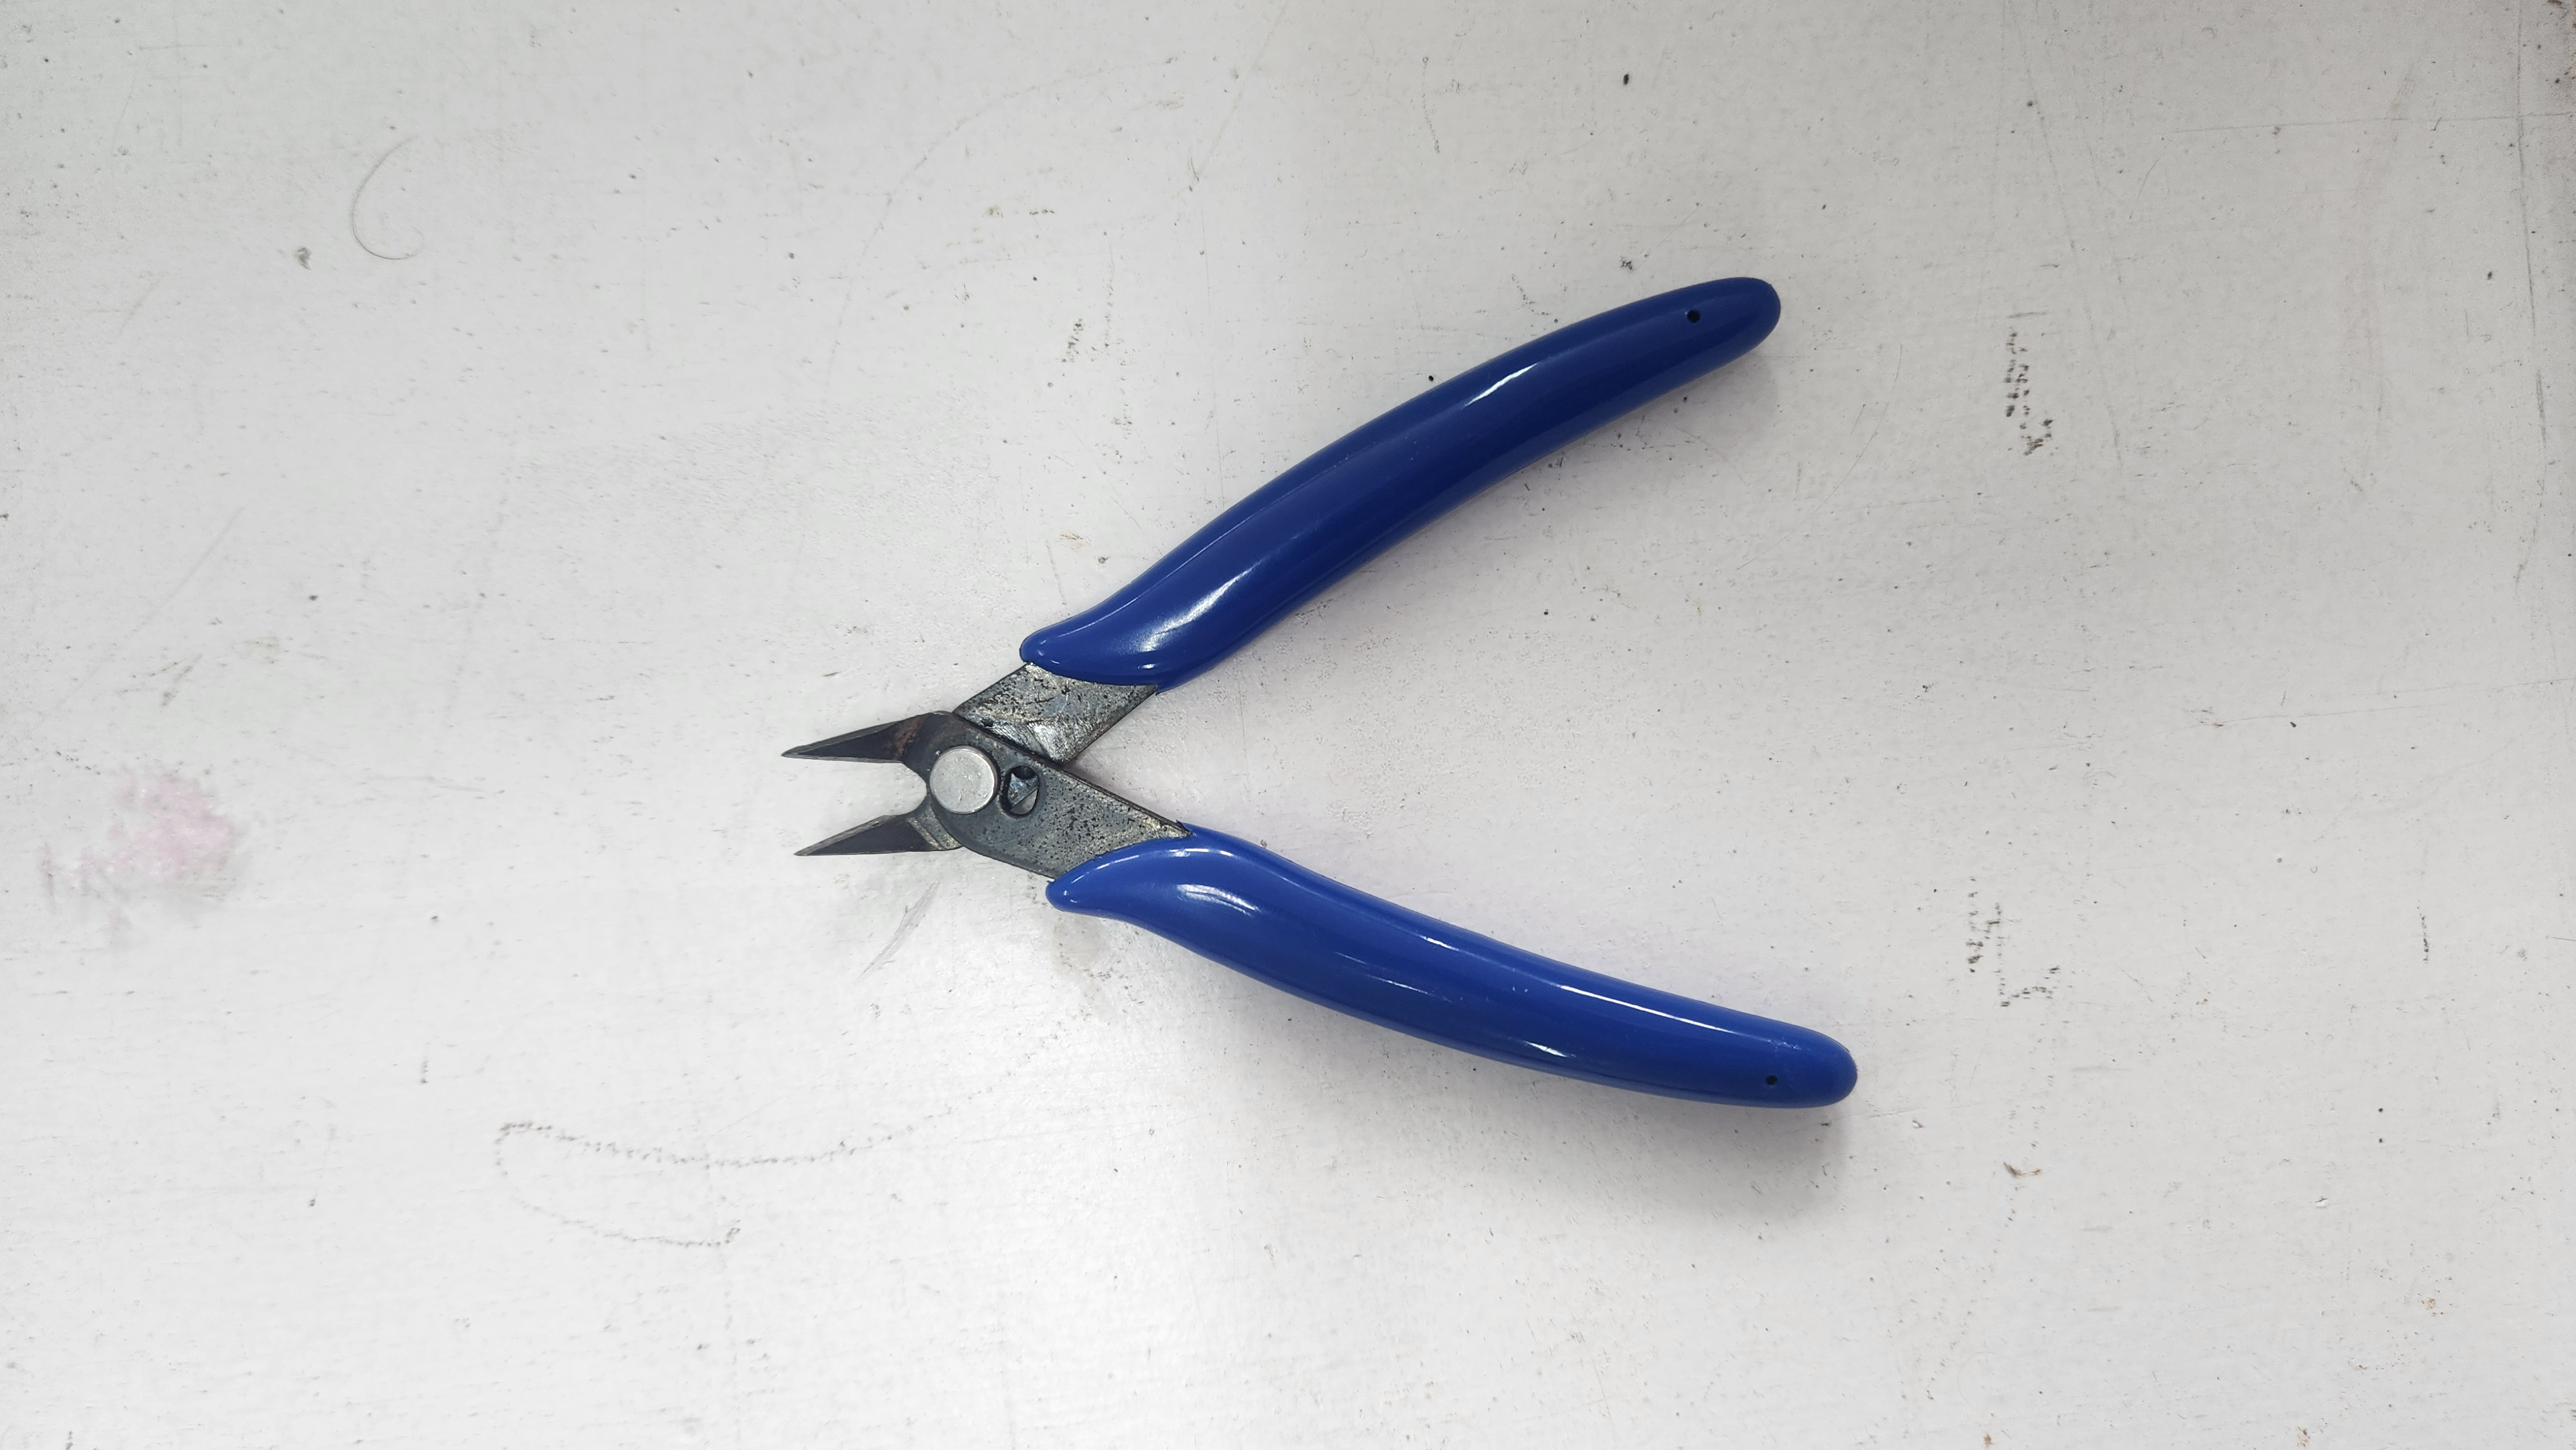
\includegraphics[width=12cm]{foto_alicate.jpg}
\caption{\label{fig:ferr_alicate}- Ferramenta de corte: Alicate.}
\end{center}
\end{figure}

\begin{figure}[H]
\begin{center}
 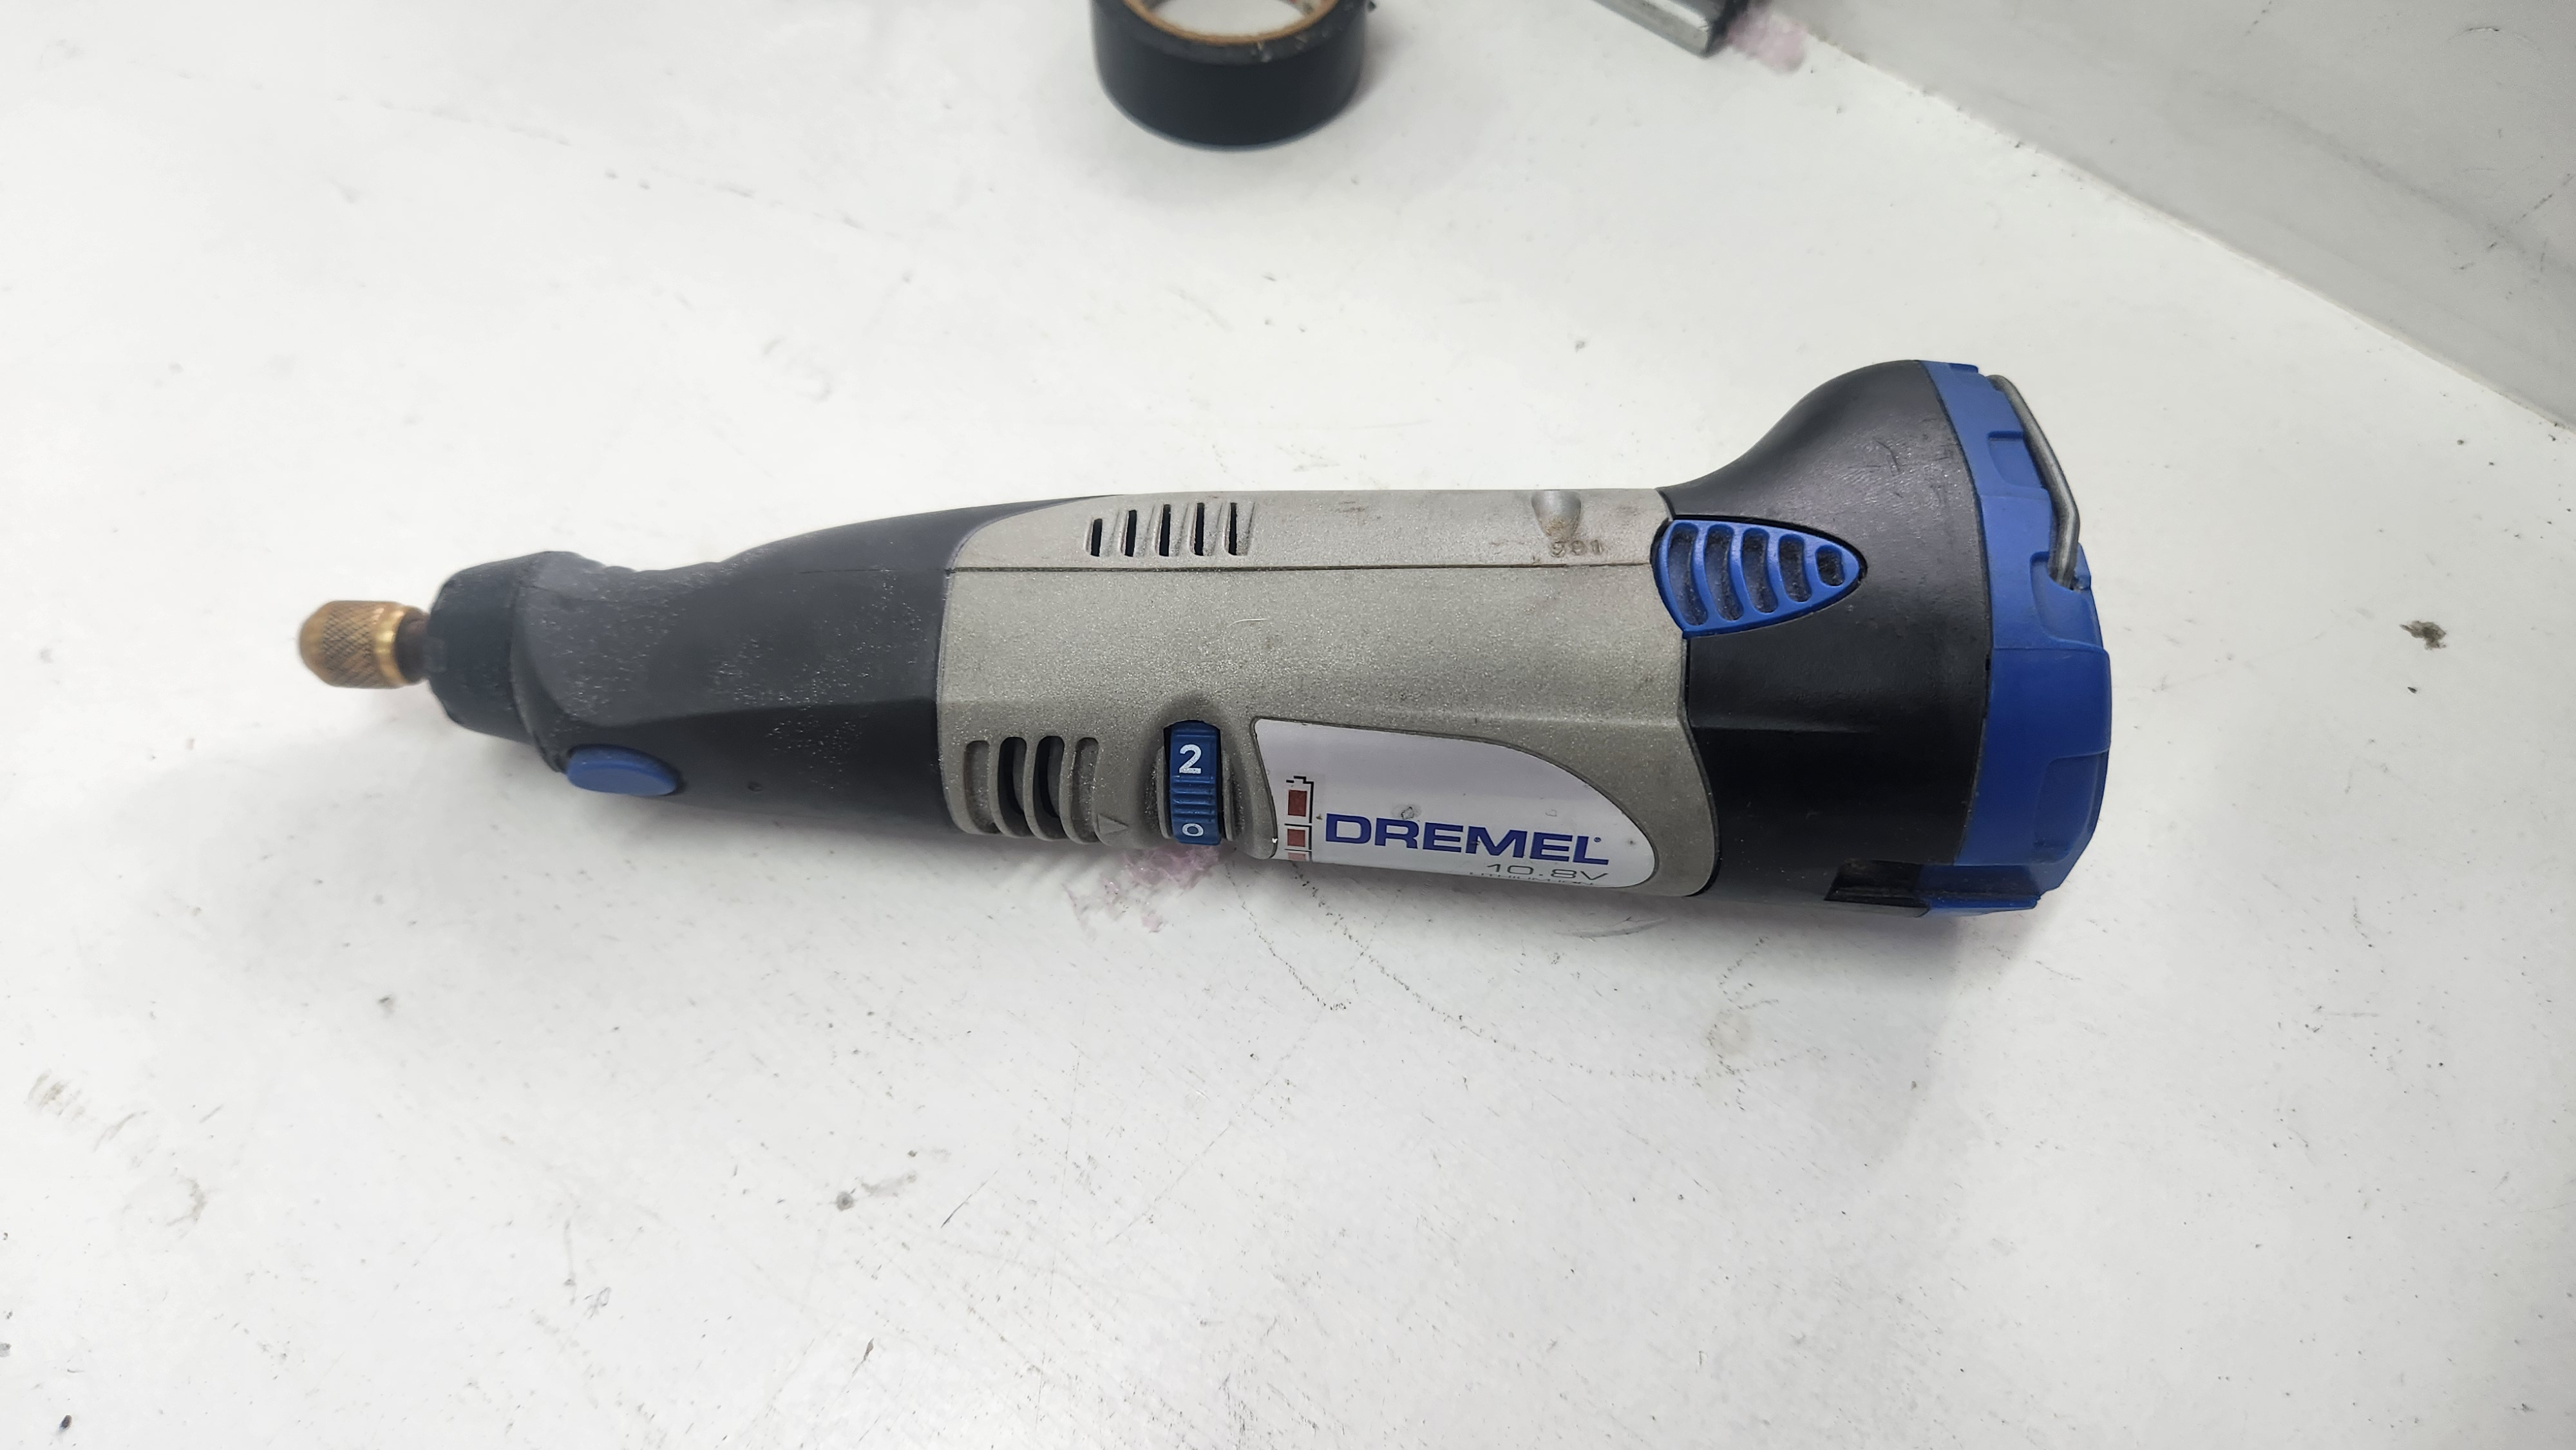
\includegraphics[width=12cm]{foto_retifica.jpg}
\caption{\label{fig:ferr_retifica}- Ferramenta de usinagem e furação: Micro retífica.}
\end{center}
\end{figure}

\begin{figure}[H]
\begin{center}
 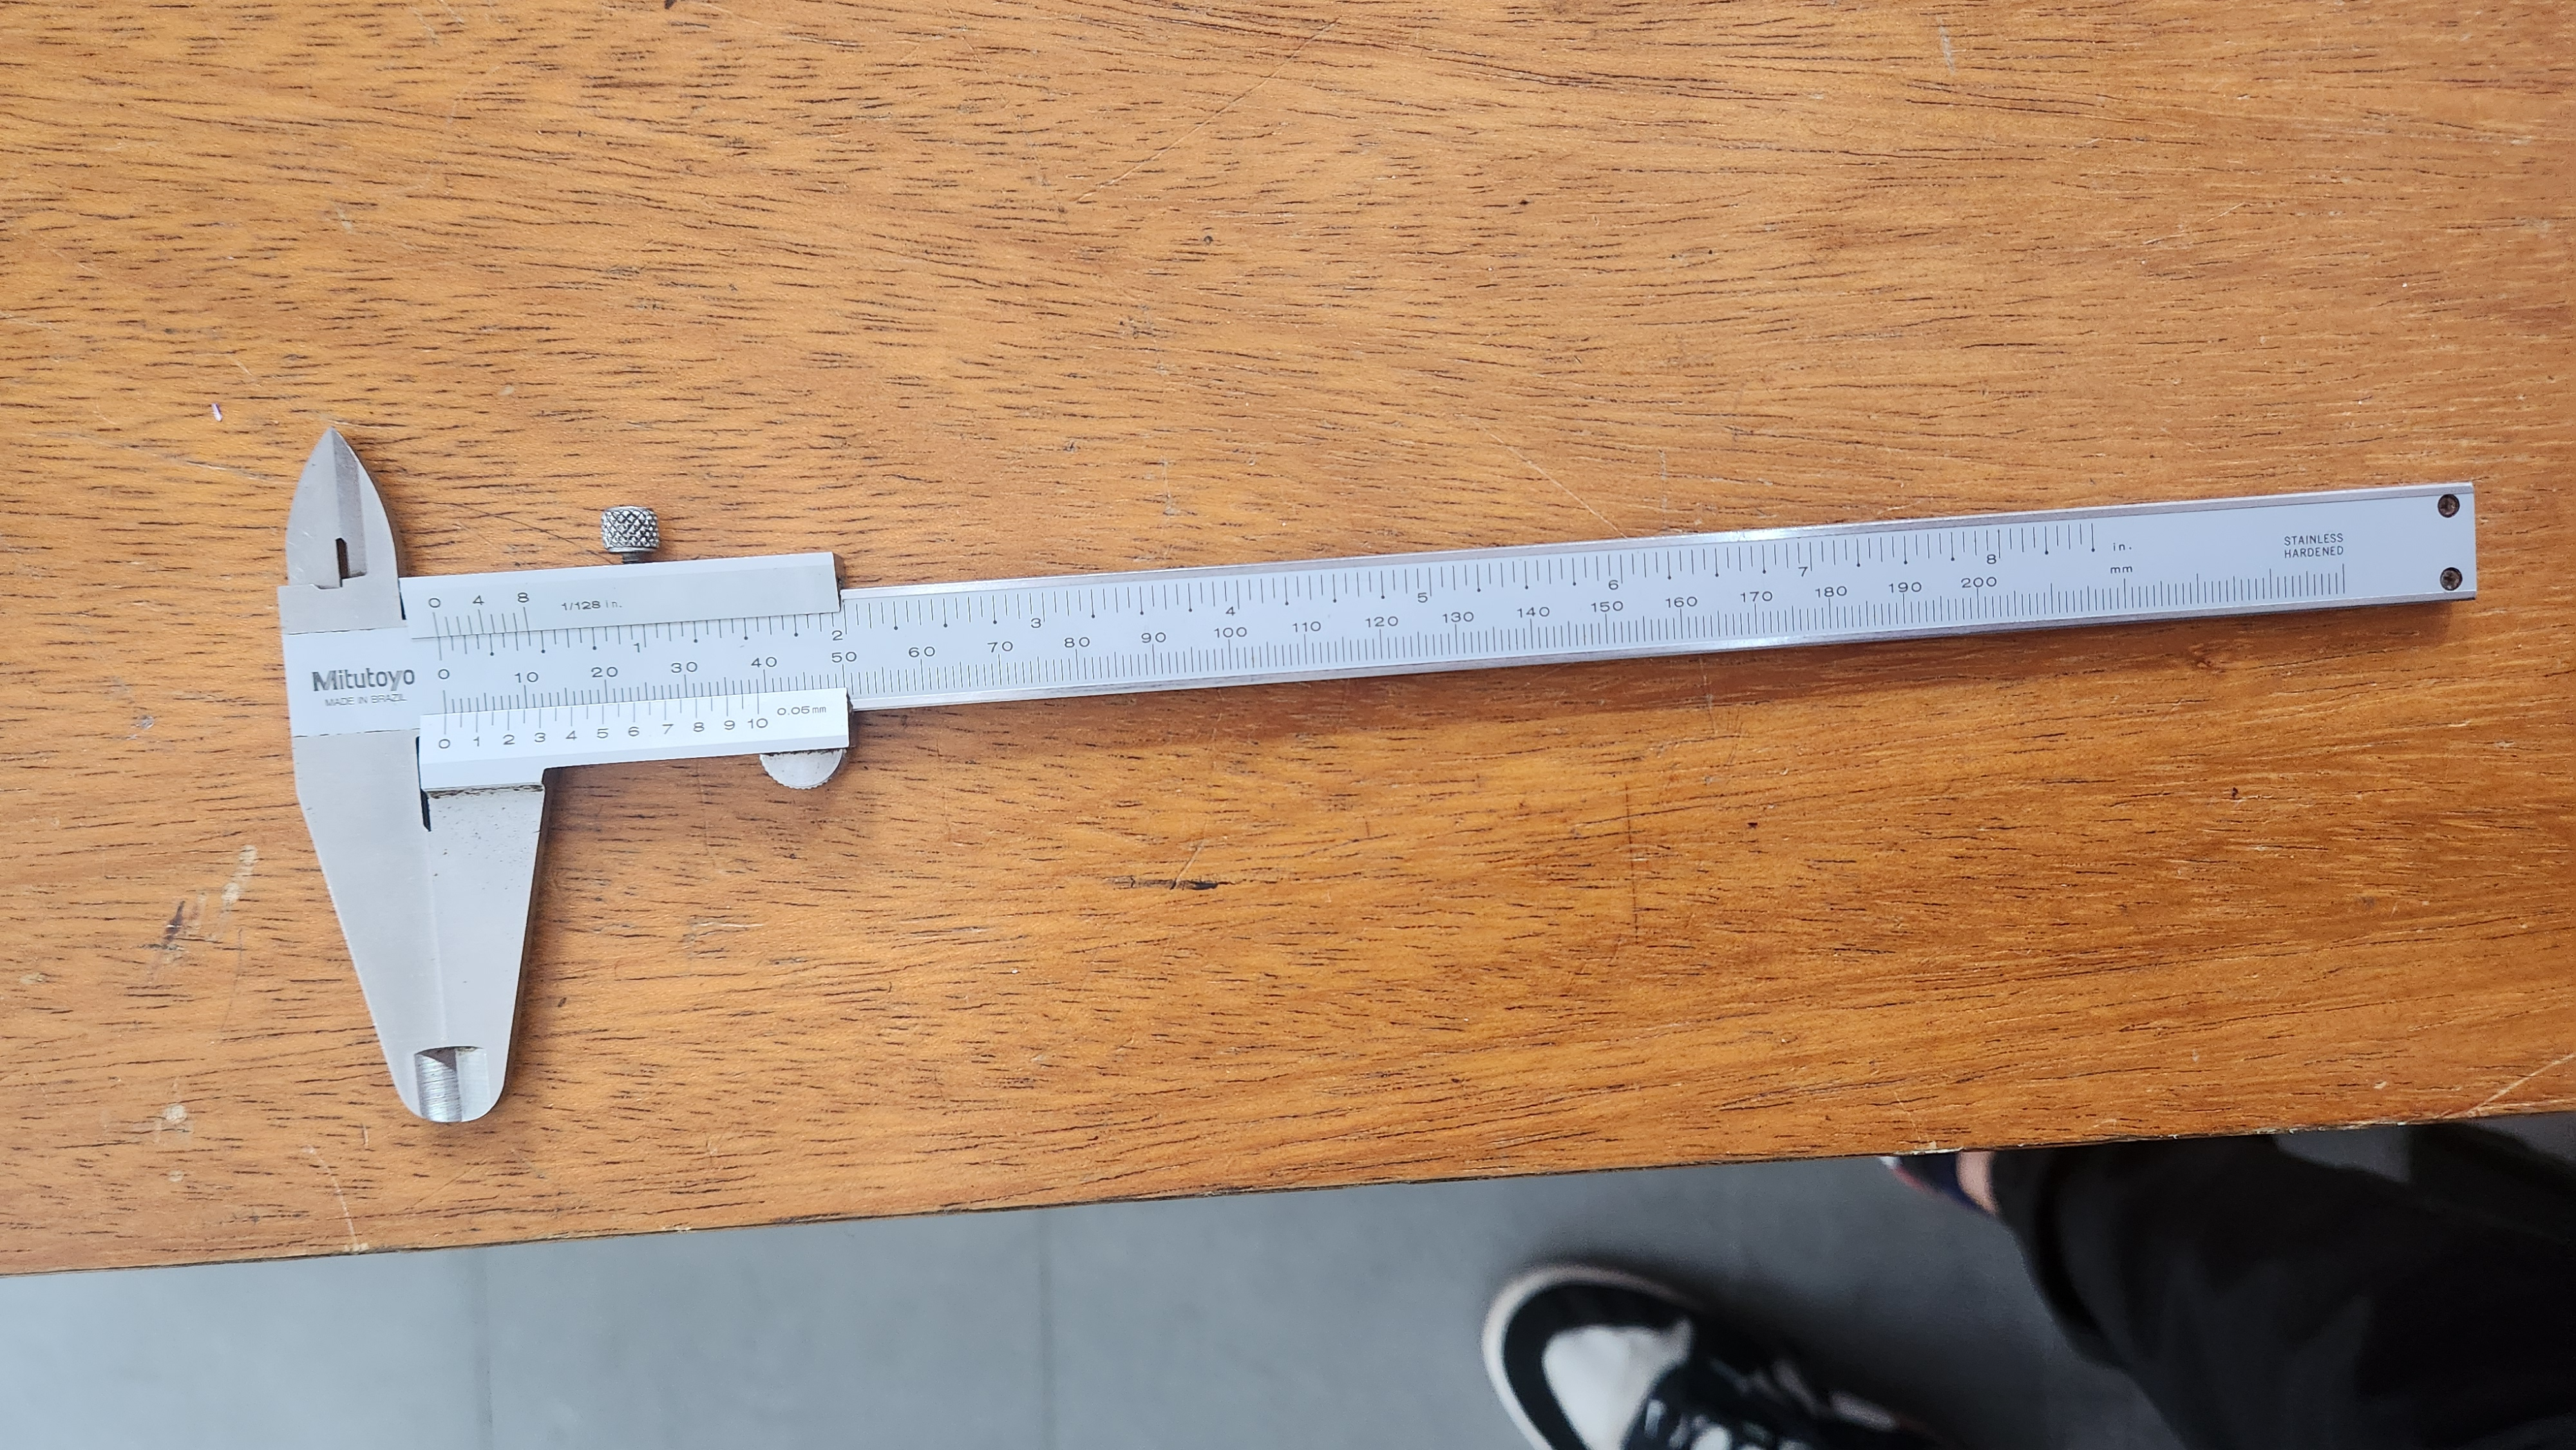
\includegraphics[width=12cm]{20261006_123529.jpg}
\caption{\label{fig:ferr_paquimetro}- Instrumento de medição: Paquímetro, de resolução de 0,05 mm, utilizado nas medidas lineares. As massas foram medidas com balança de precisão.}
\end{center}
\end{figure}

\section{Parâmetros Geométricos e Inerciais das Peças}
\label{sec:parametros}

A exatidão do modelo dinâmico depende diretamente das propriedades físicas de cada corpo rígido que compõe o mecanismo. O robô apresenta simetria em grande parte de sua estrutura, sendo subdividido analiticamente em 4 conjuntos de peças de madeira (Ombro, Quadril, Braço e Perna), aos quais se somam o motor com caixa de redução e a bateria, que formam o chassi. 

Para a aplicação das equações de movimento, levantou-se a massa individual de cada componente utilizando uma balança de precisão. Esses valores são fundamentais para o cálculo dos centros de massa e do tensor de inércia, e estão consolidados na \ref{tab:pesos_partes}. A massa da bateria foi medida; a do motor com caixa de redução foi medida em 26,6 g.

\begin{table}[H]
\centering
\caption{\label{tab:pesos_partes}- Massa individual das partes constituintes do robô.}
\vspace*{.1cm}
\begin{tabular}{|c|l|c|}
\hline
\textbf{Ref. Visual} & \textbf{Descrição do Componente} & \textbf{Massa (g)}\\
\hline
Fig. 1 e 2 & Ombro & 0,83 \\ 
\hline
Fig. 3 & Quadril & 0,81 \\
\hline
Fig. 4 & Braço & 2,0 \\
\hline
Fig. 5 e 6 & Perna & 1,5 \\
\hline
Fig. \ref{fig:desenho_motor} & Motor com caixa de redução (massa medida) & 26,6 \\
\hline
--- & Bateria & 67,03 \\
\hline
\end{tabular}
\end{table}

\subsection{Detalhamento Físico das Partes Móveis}

Além das massas, os comprimentos efetivos de cada elo foram medidos para a definição exata dos vetores posição ($\vec{r}_{B/A}$) utilizados nas equações cinemáticas. Devido à geometria 3D das peças, algumas exigiram documentação em mais de um plano. A seguir, são apresentadas as fotografias detalhadas das partes isoladas, evidenciando suas respectivas cotas dimensionais nas visões lateral e frontal.

\begin{figure}[H]
\begin{center}
 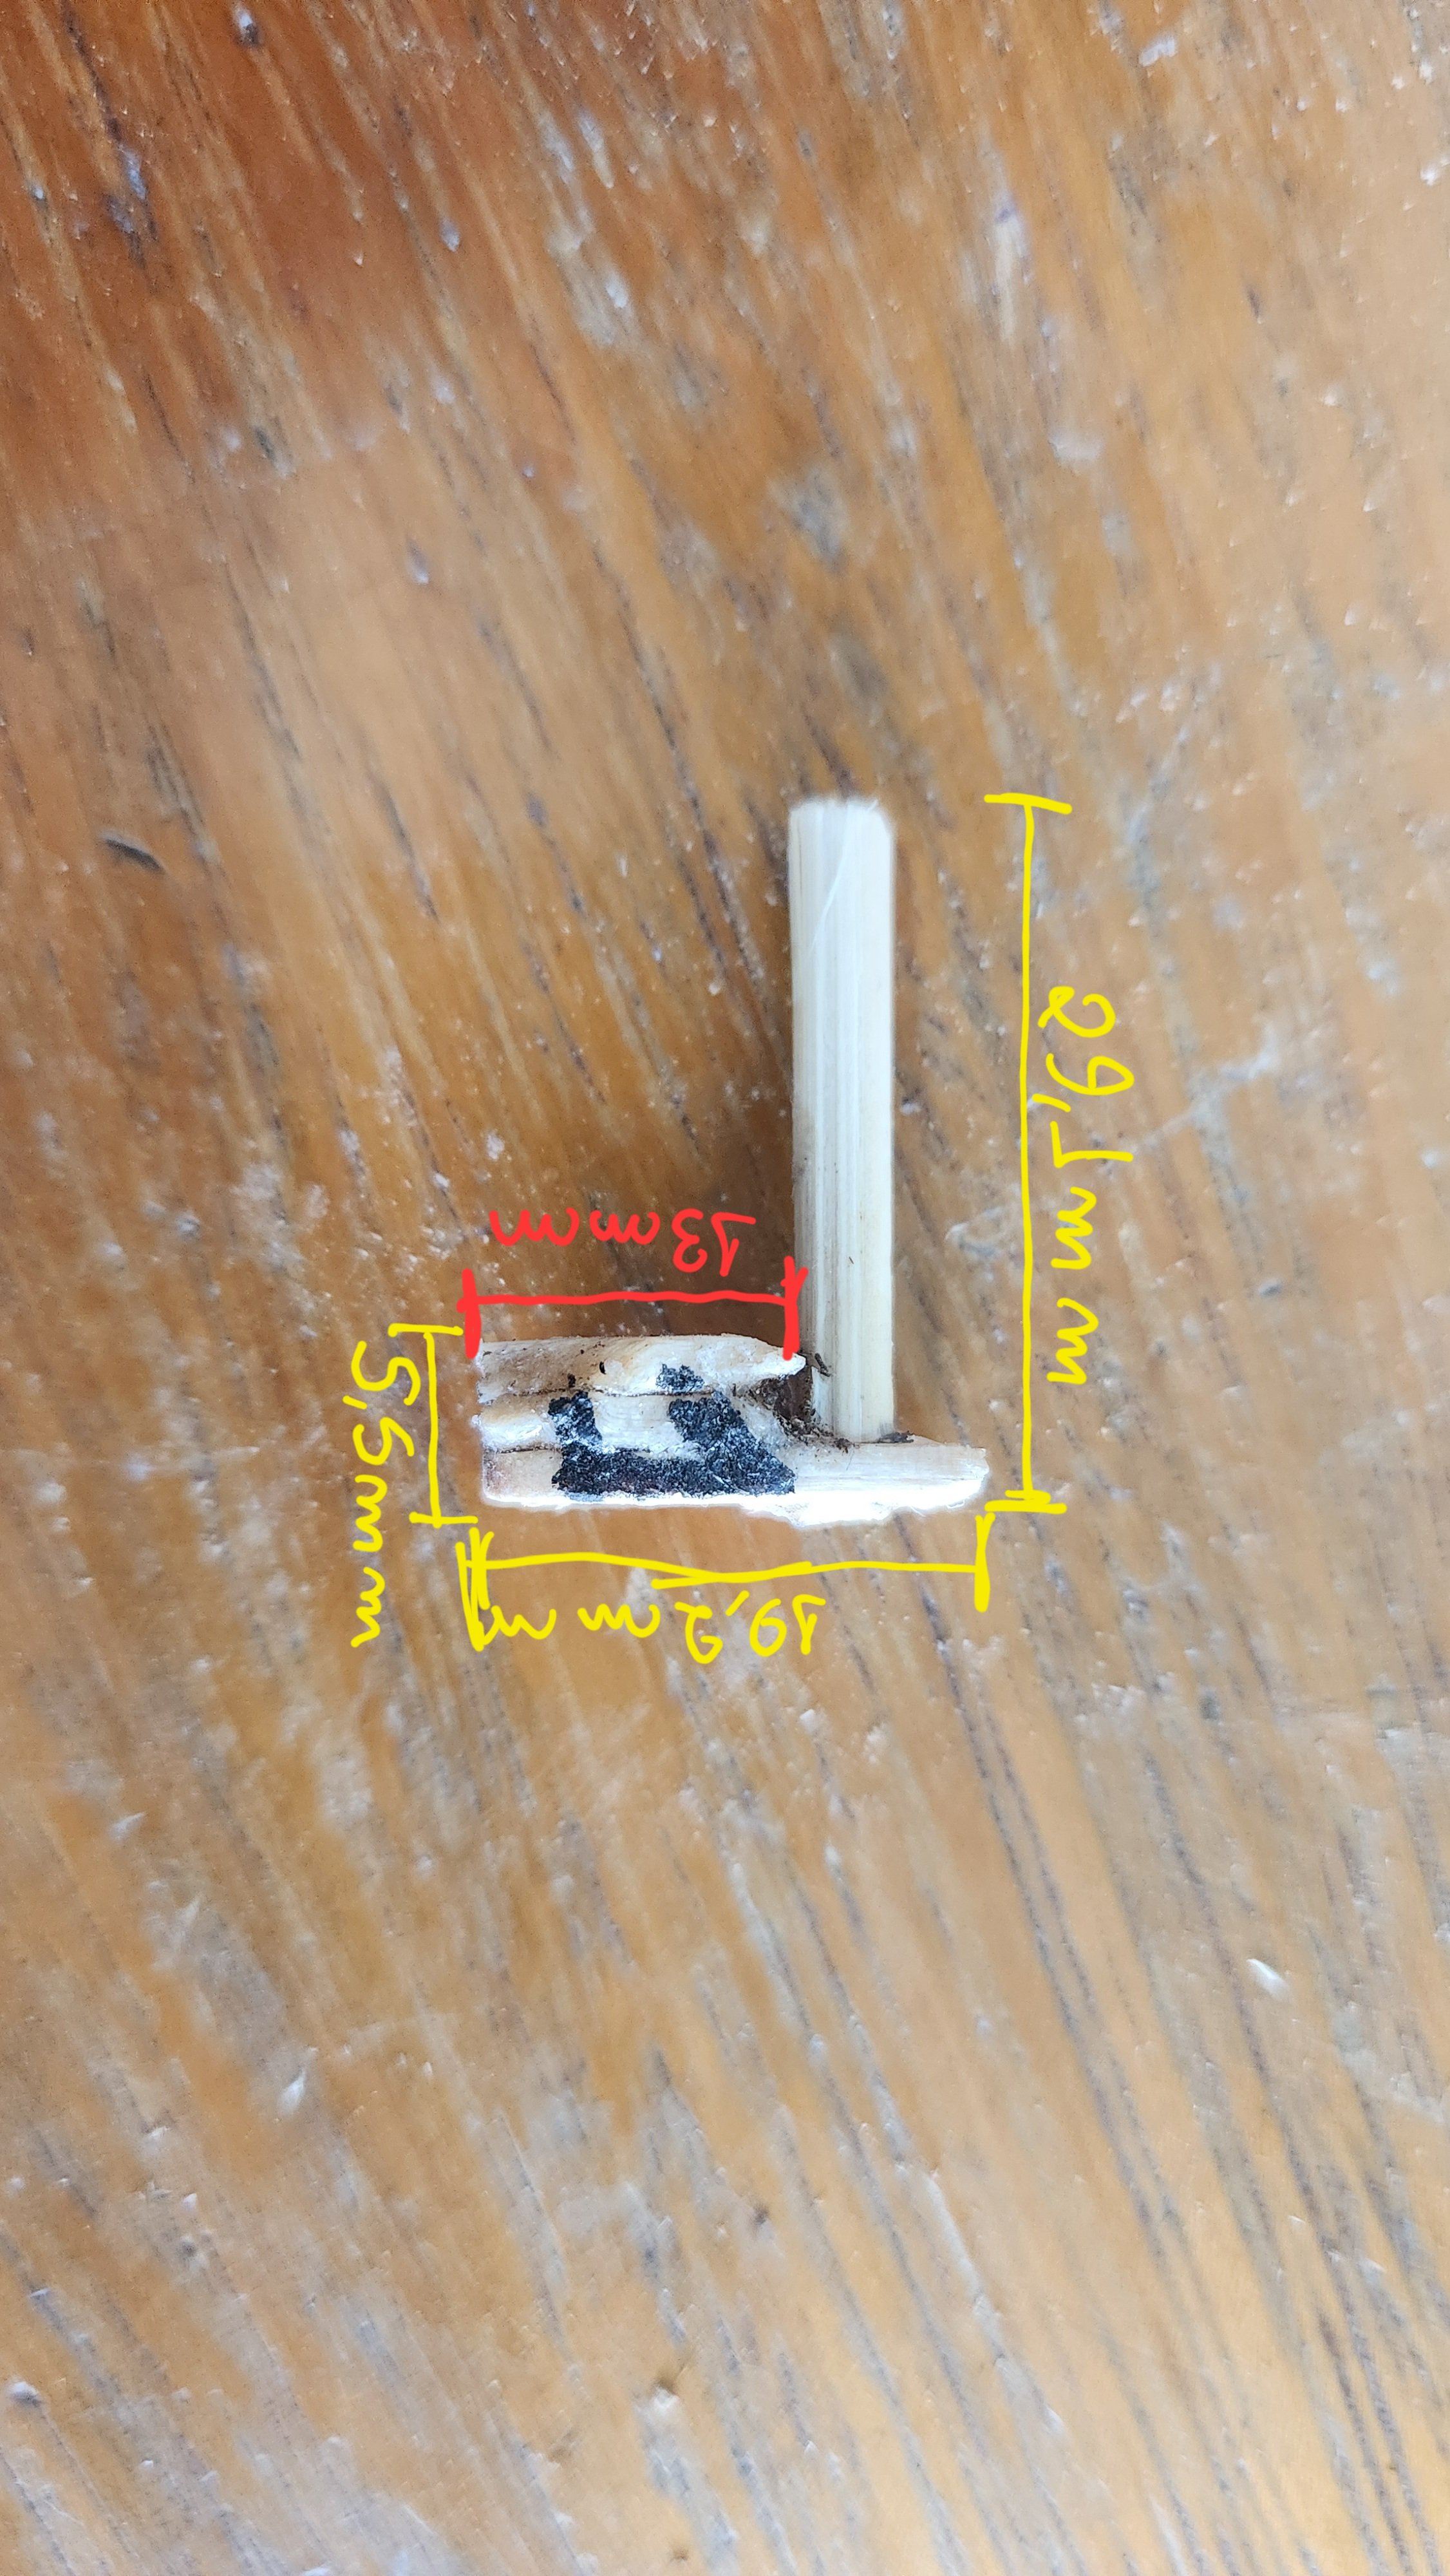
\includegraphics[width=10cm]{foto_parte1.jpg} % Lembre-se de ajustar o caminho da pasta se necessário, ex: ./03_Cap2/foto_parte1.jpg
\caption{\label{fig:parte1}- Detalhe e dimensões do Ombro (visão lateral).}
\end{center}
\end{figure}

\begin{figure}[H]
\begin{center}
 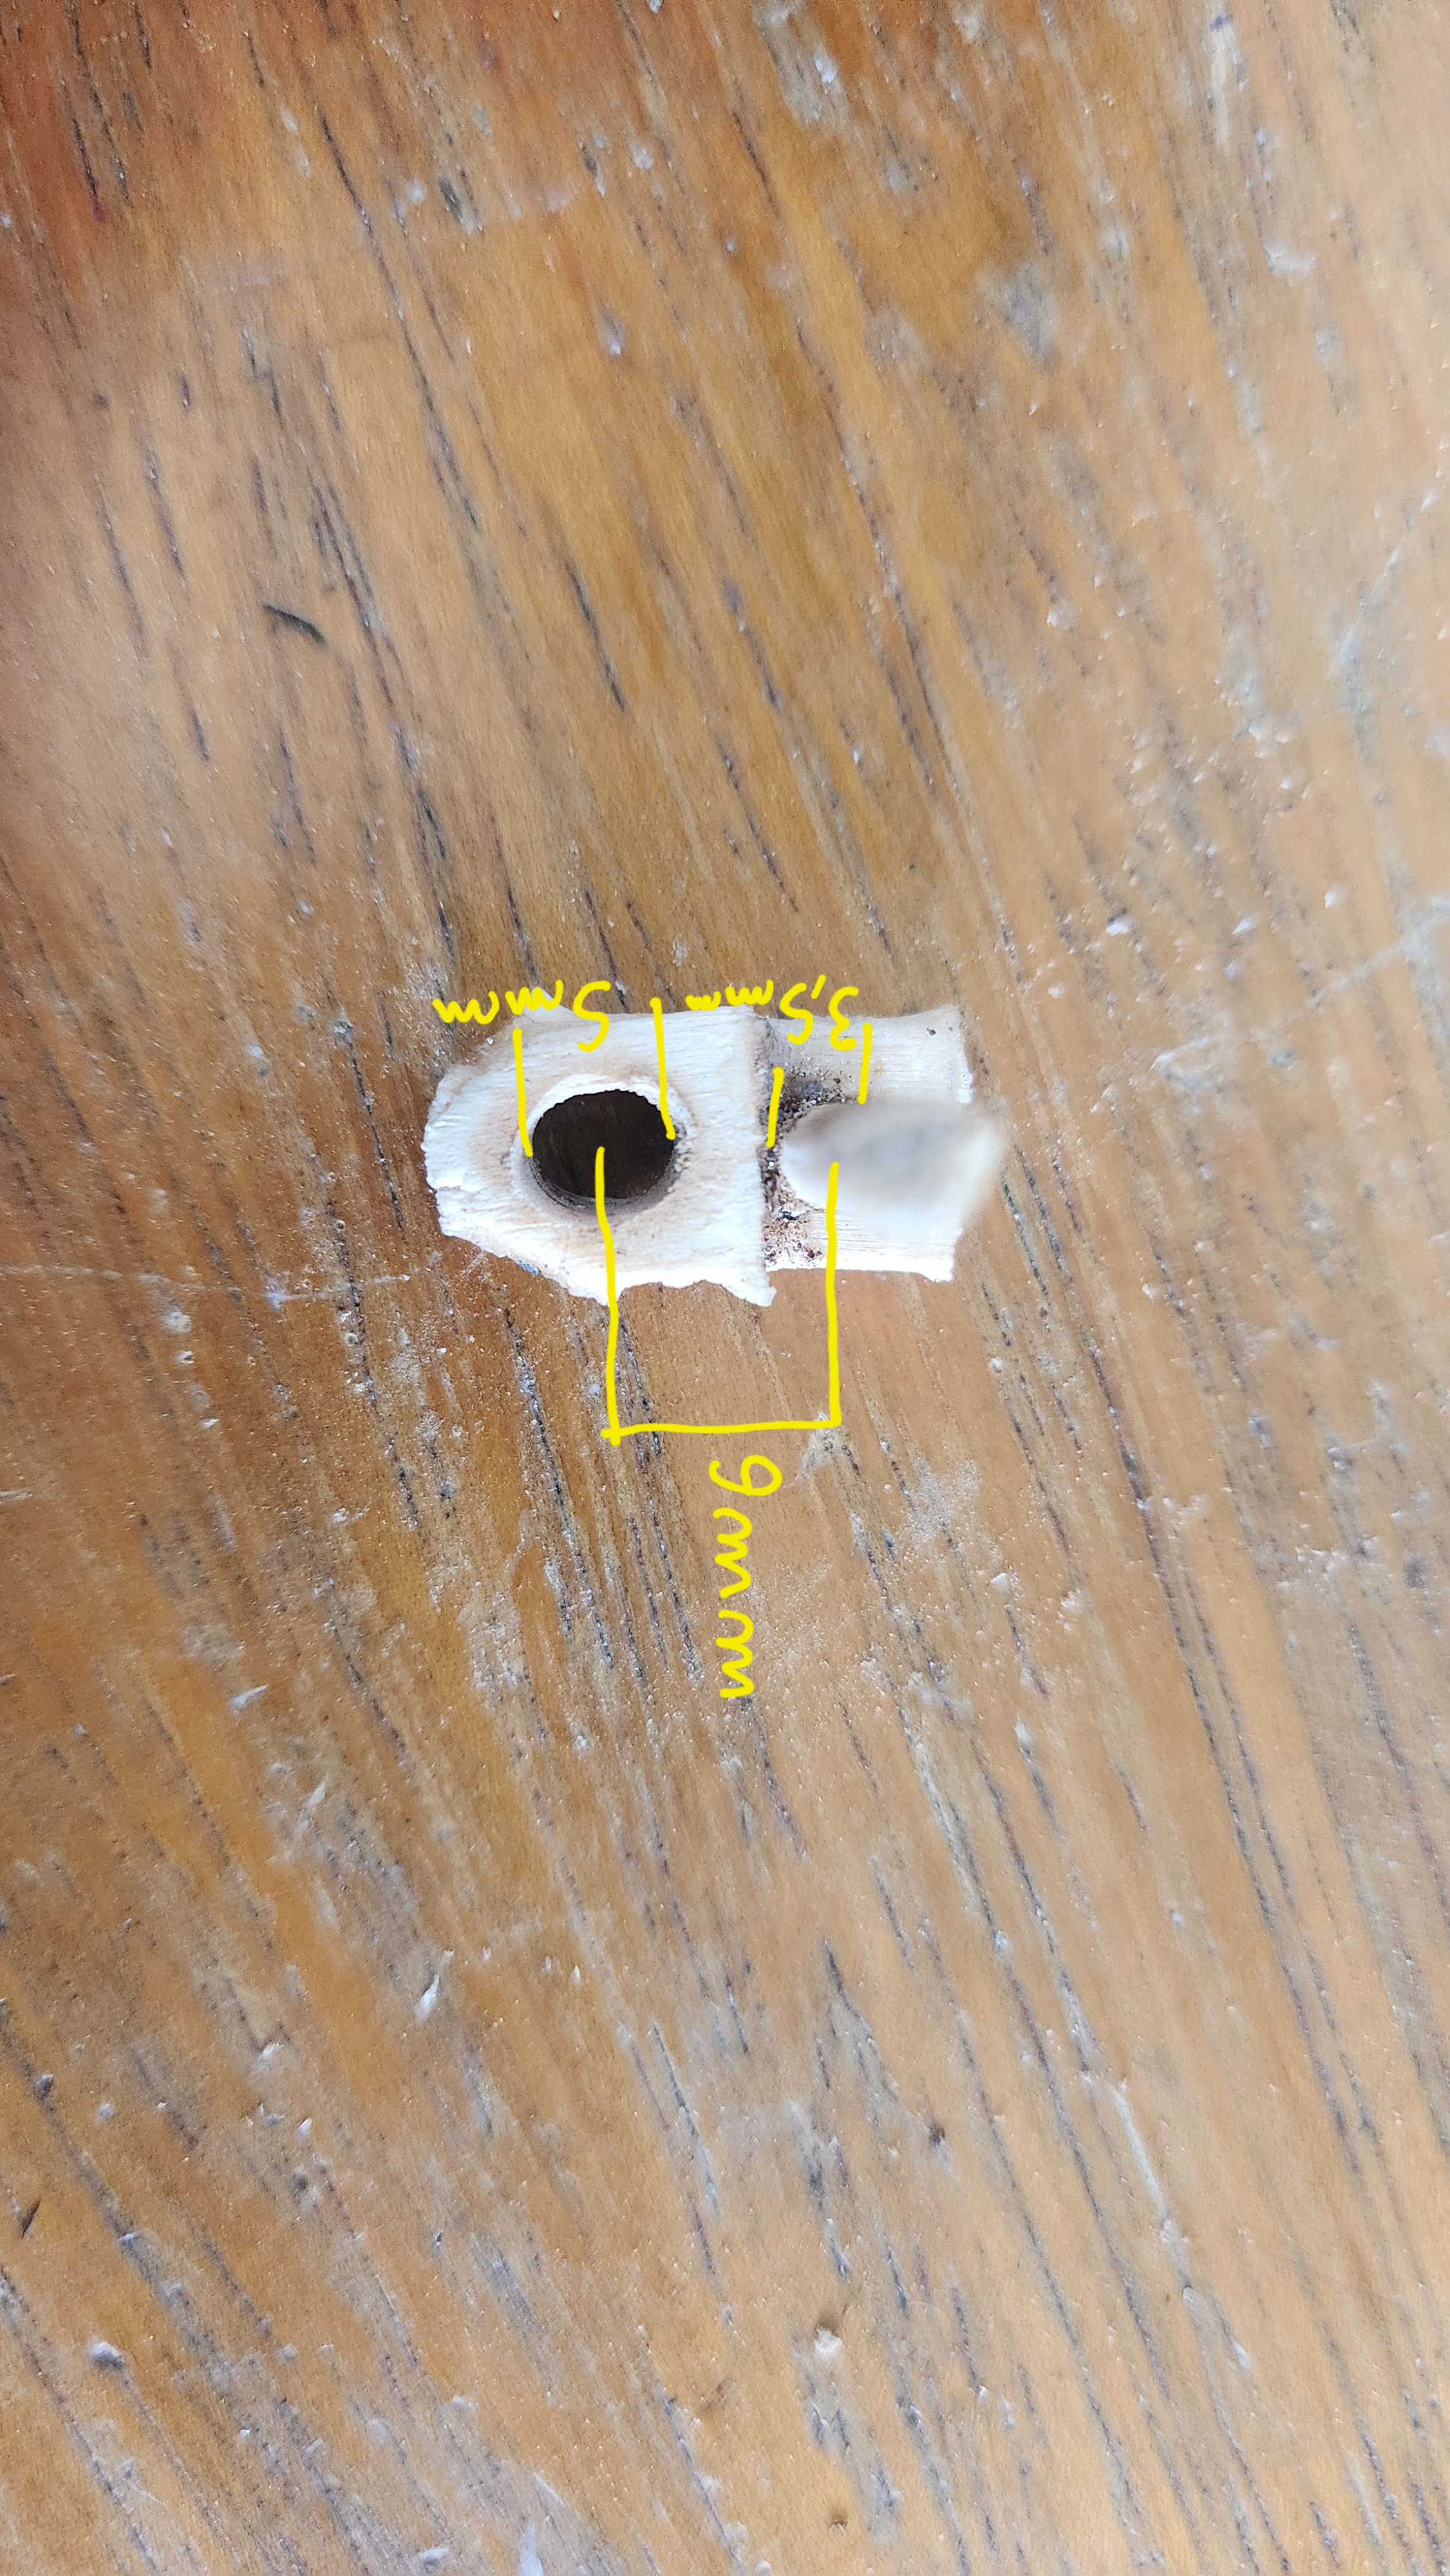
\includegraphics[width=10cm]{foto_parte2.jpg}
\caption{\label{fig:parte2}- Detalhe e dimensões do Ombro (visão frontal).}
\end{center}
\end{figure}

\begin{figure}[H]
\begin{center}
 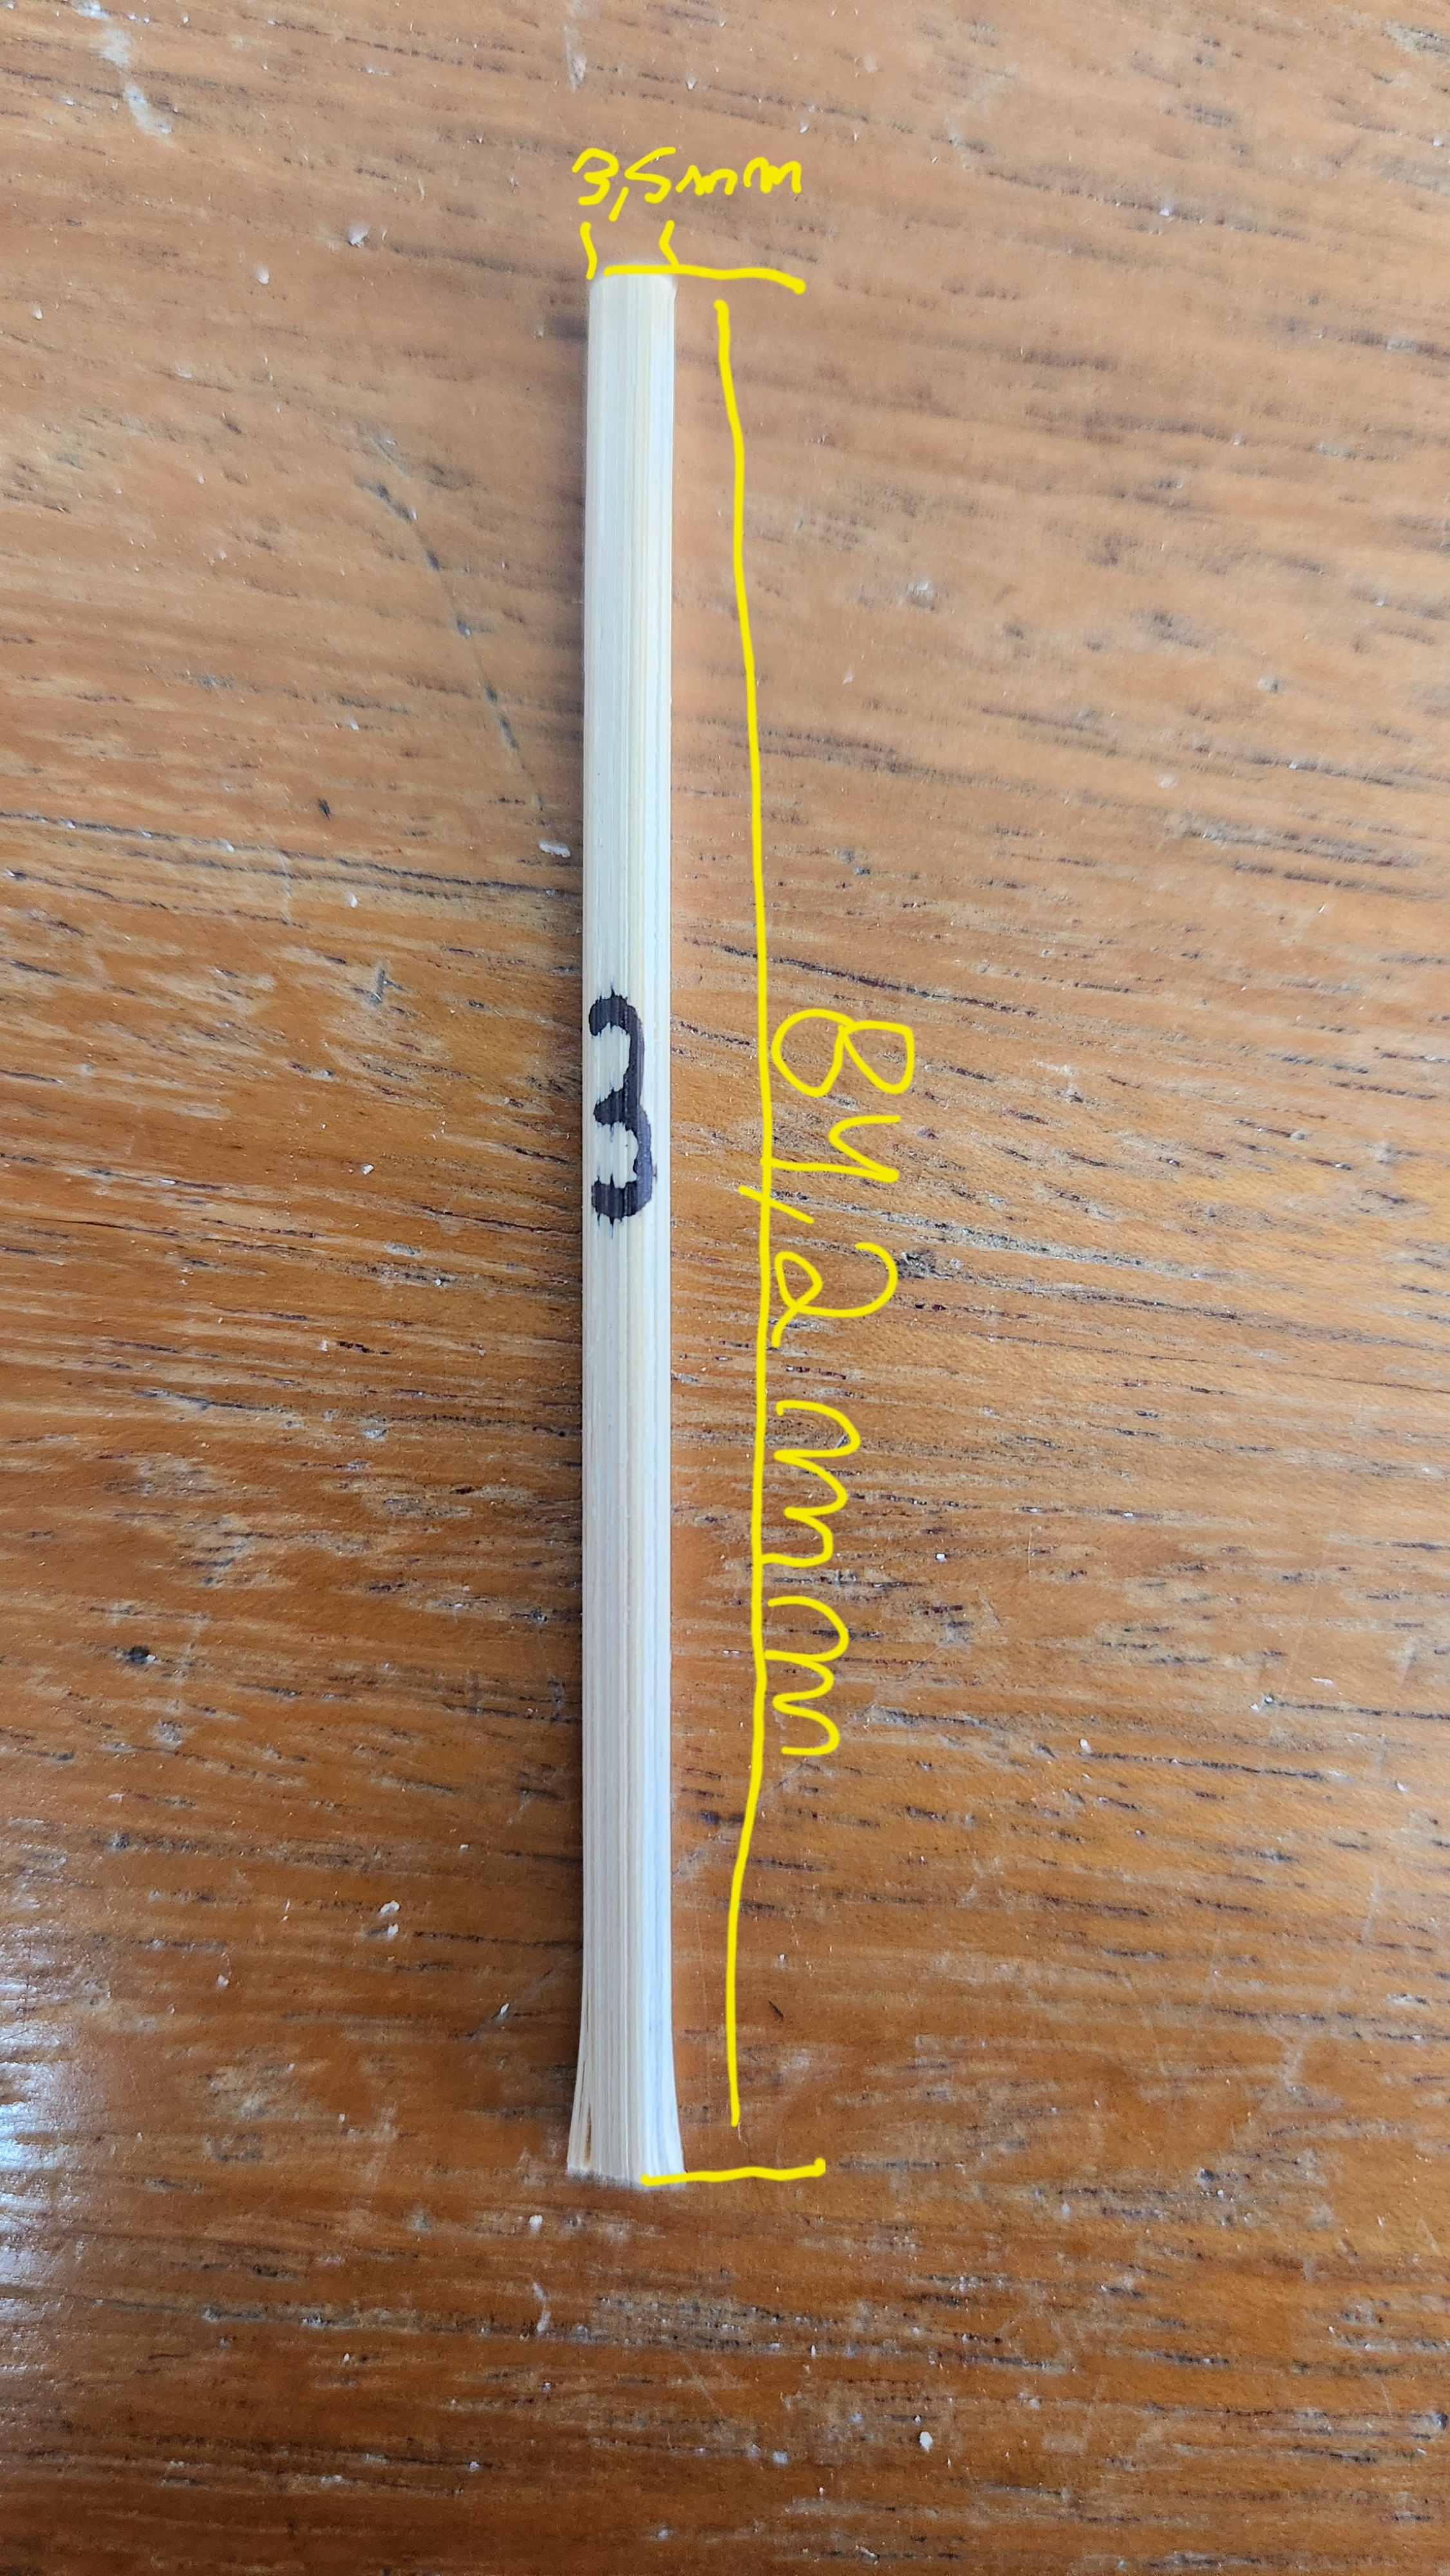
\includegraphics[width=10cm]{foto_parte3.jpg}
\caption{\label{fig:parte3}- Detalhe e dimensões do Quadril.}
\end{center}
\end{figure}

\begin{figure}[H]
\begin{center}
 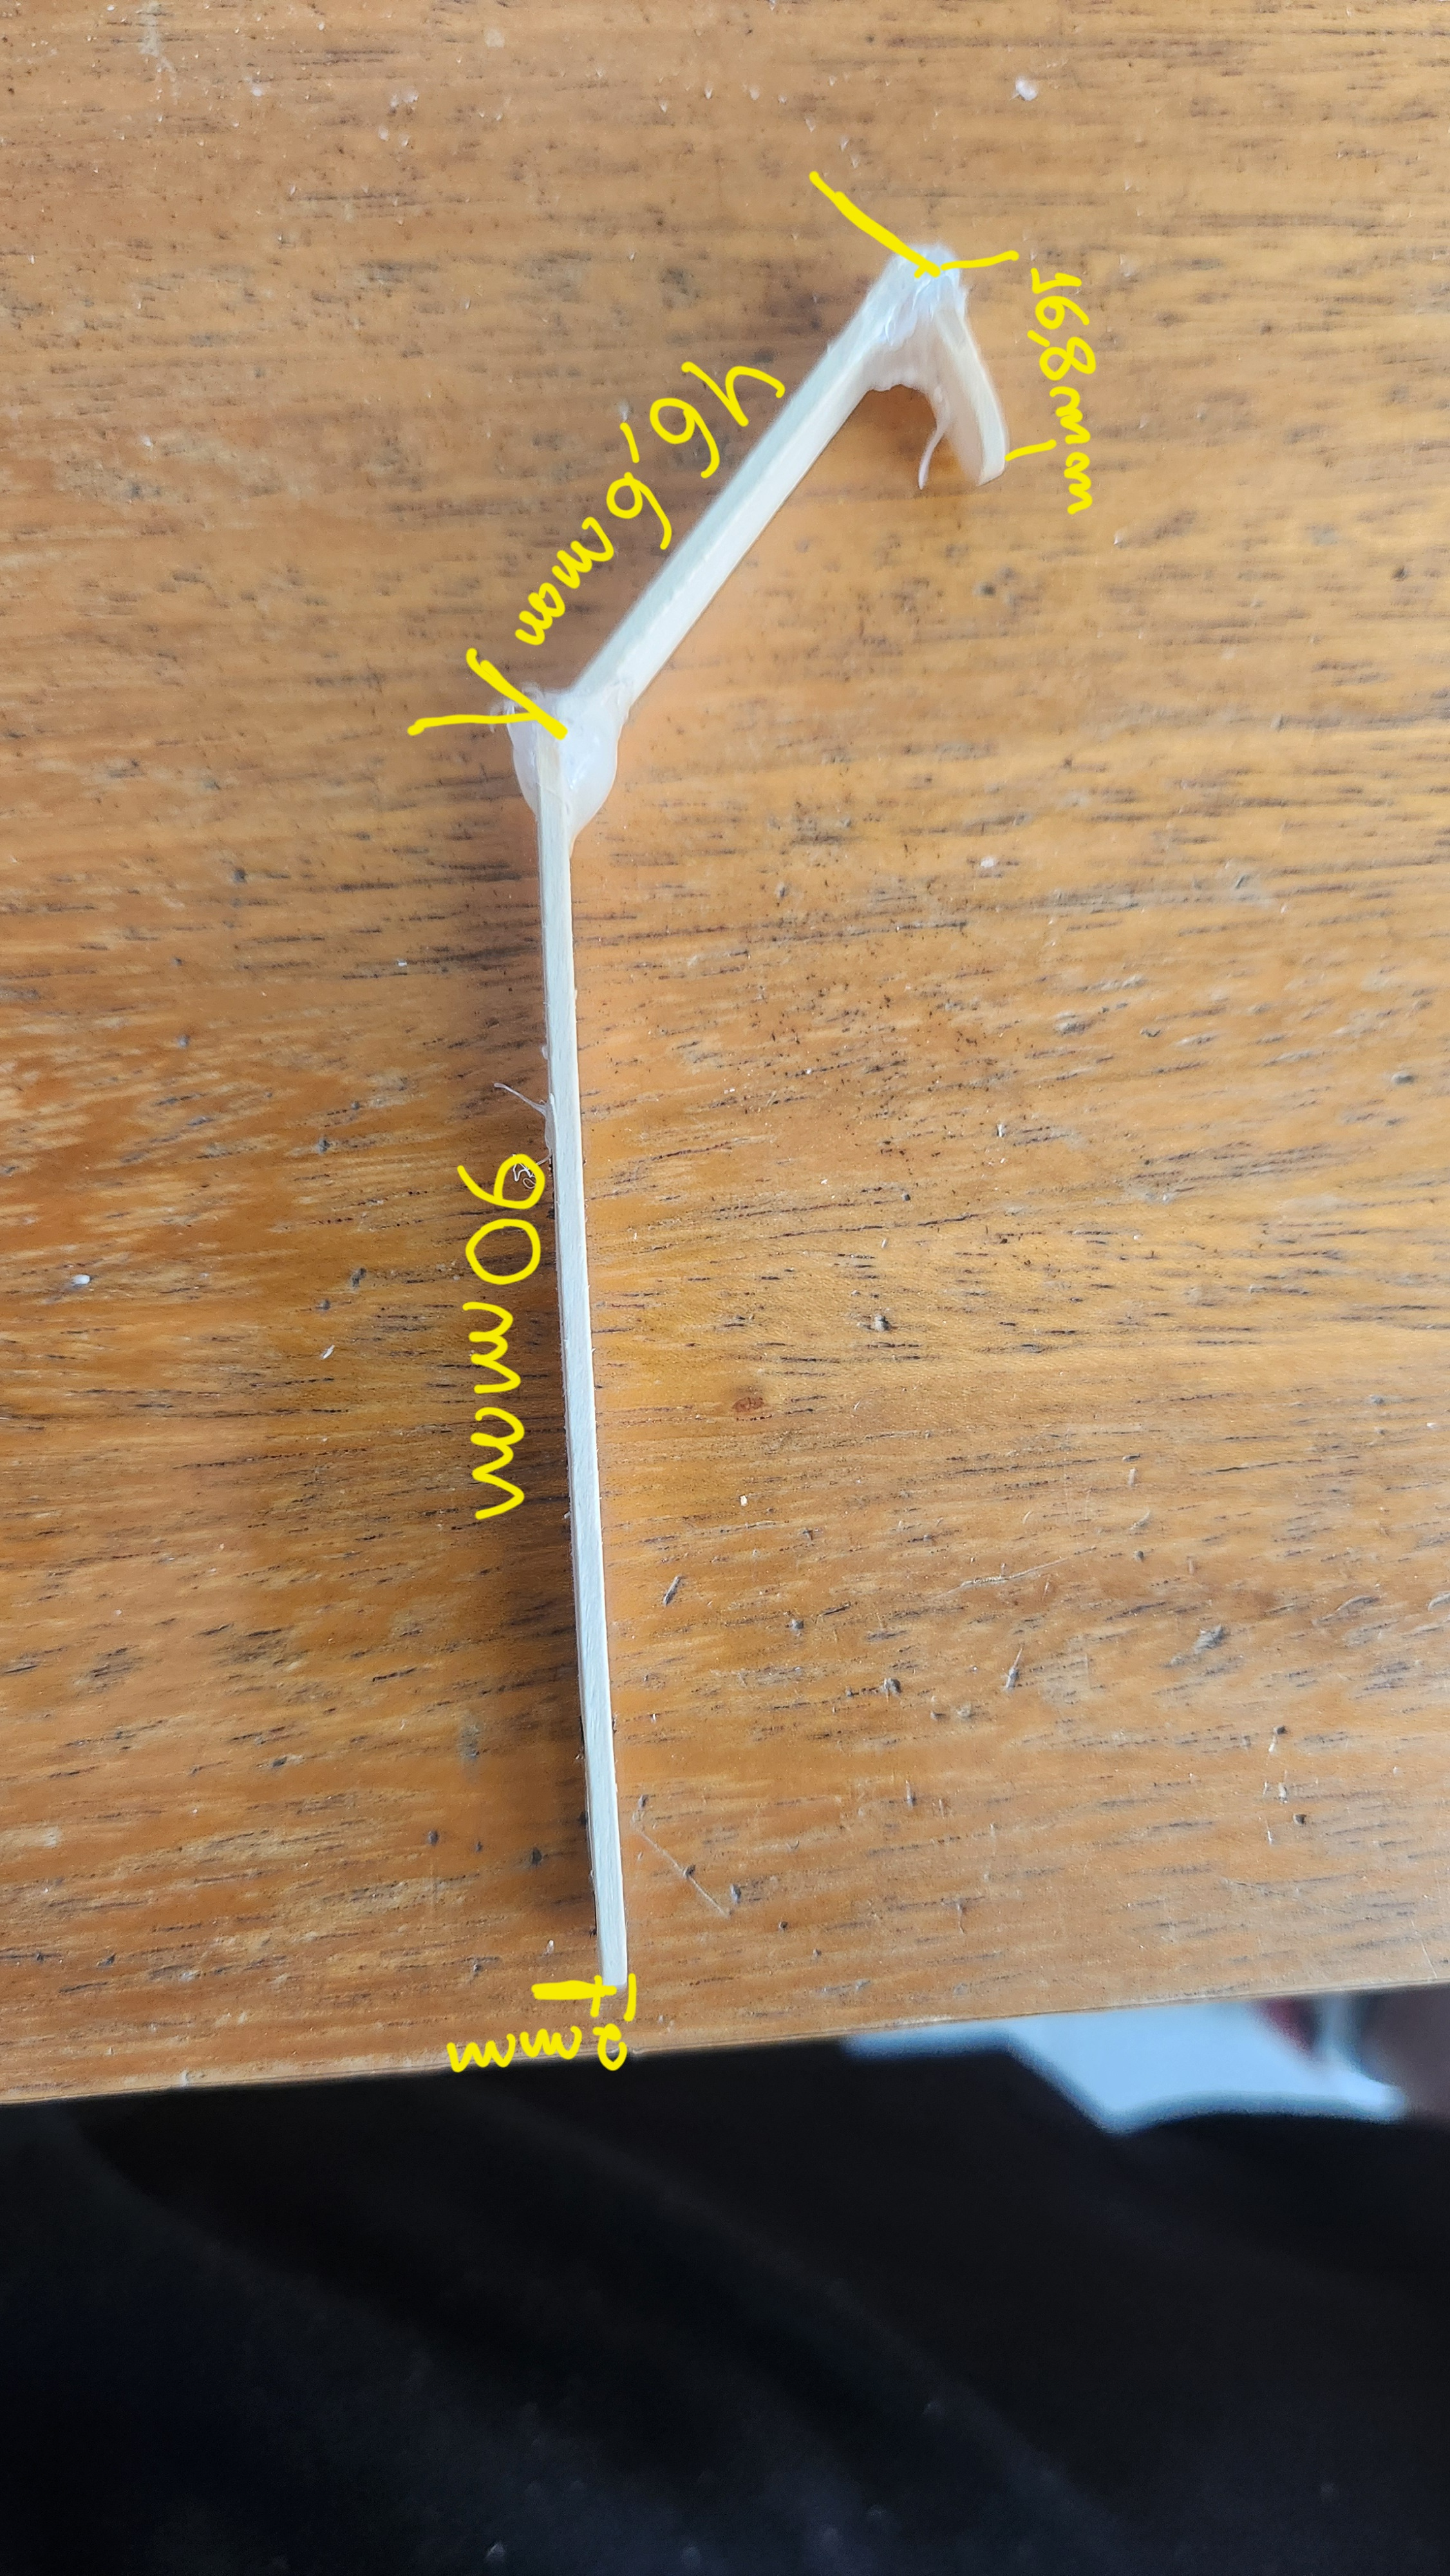
\includegraphics[width=10cm]{foto_parte4.jpg}
\caption{\label{fig:parte4}- Detalhe e dimensões do Braço.}
\end{center}
\end{figure}

\begin{figure}[H]
\begin{center}
 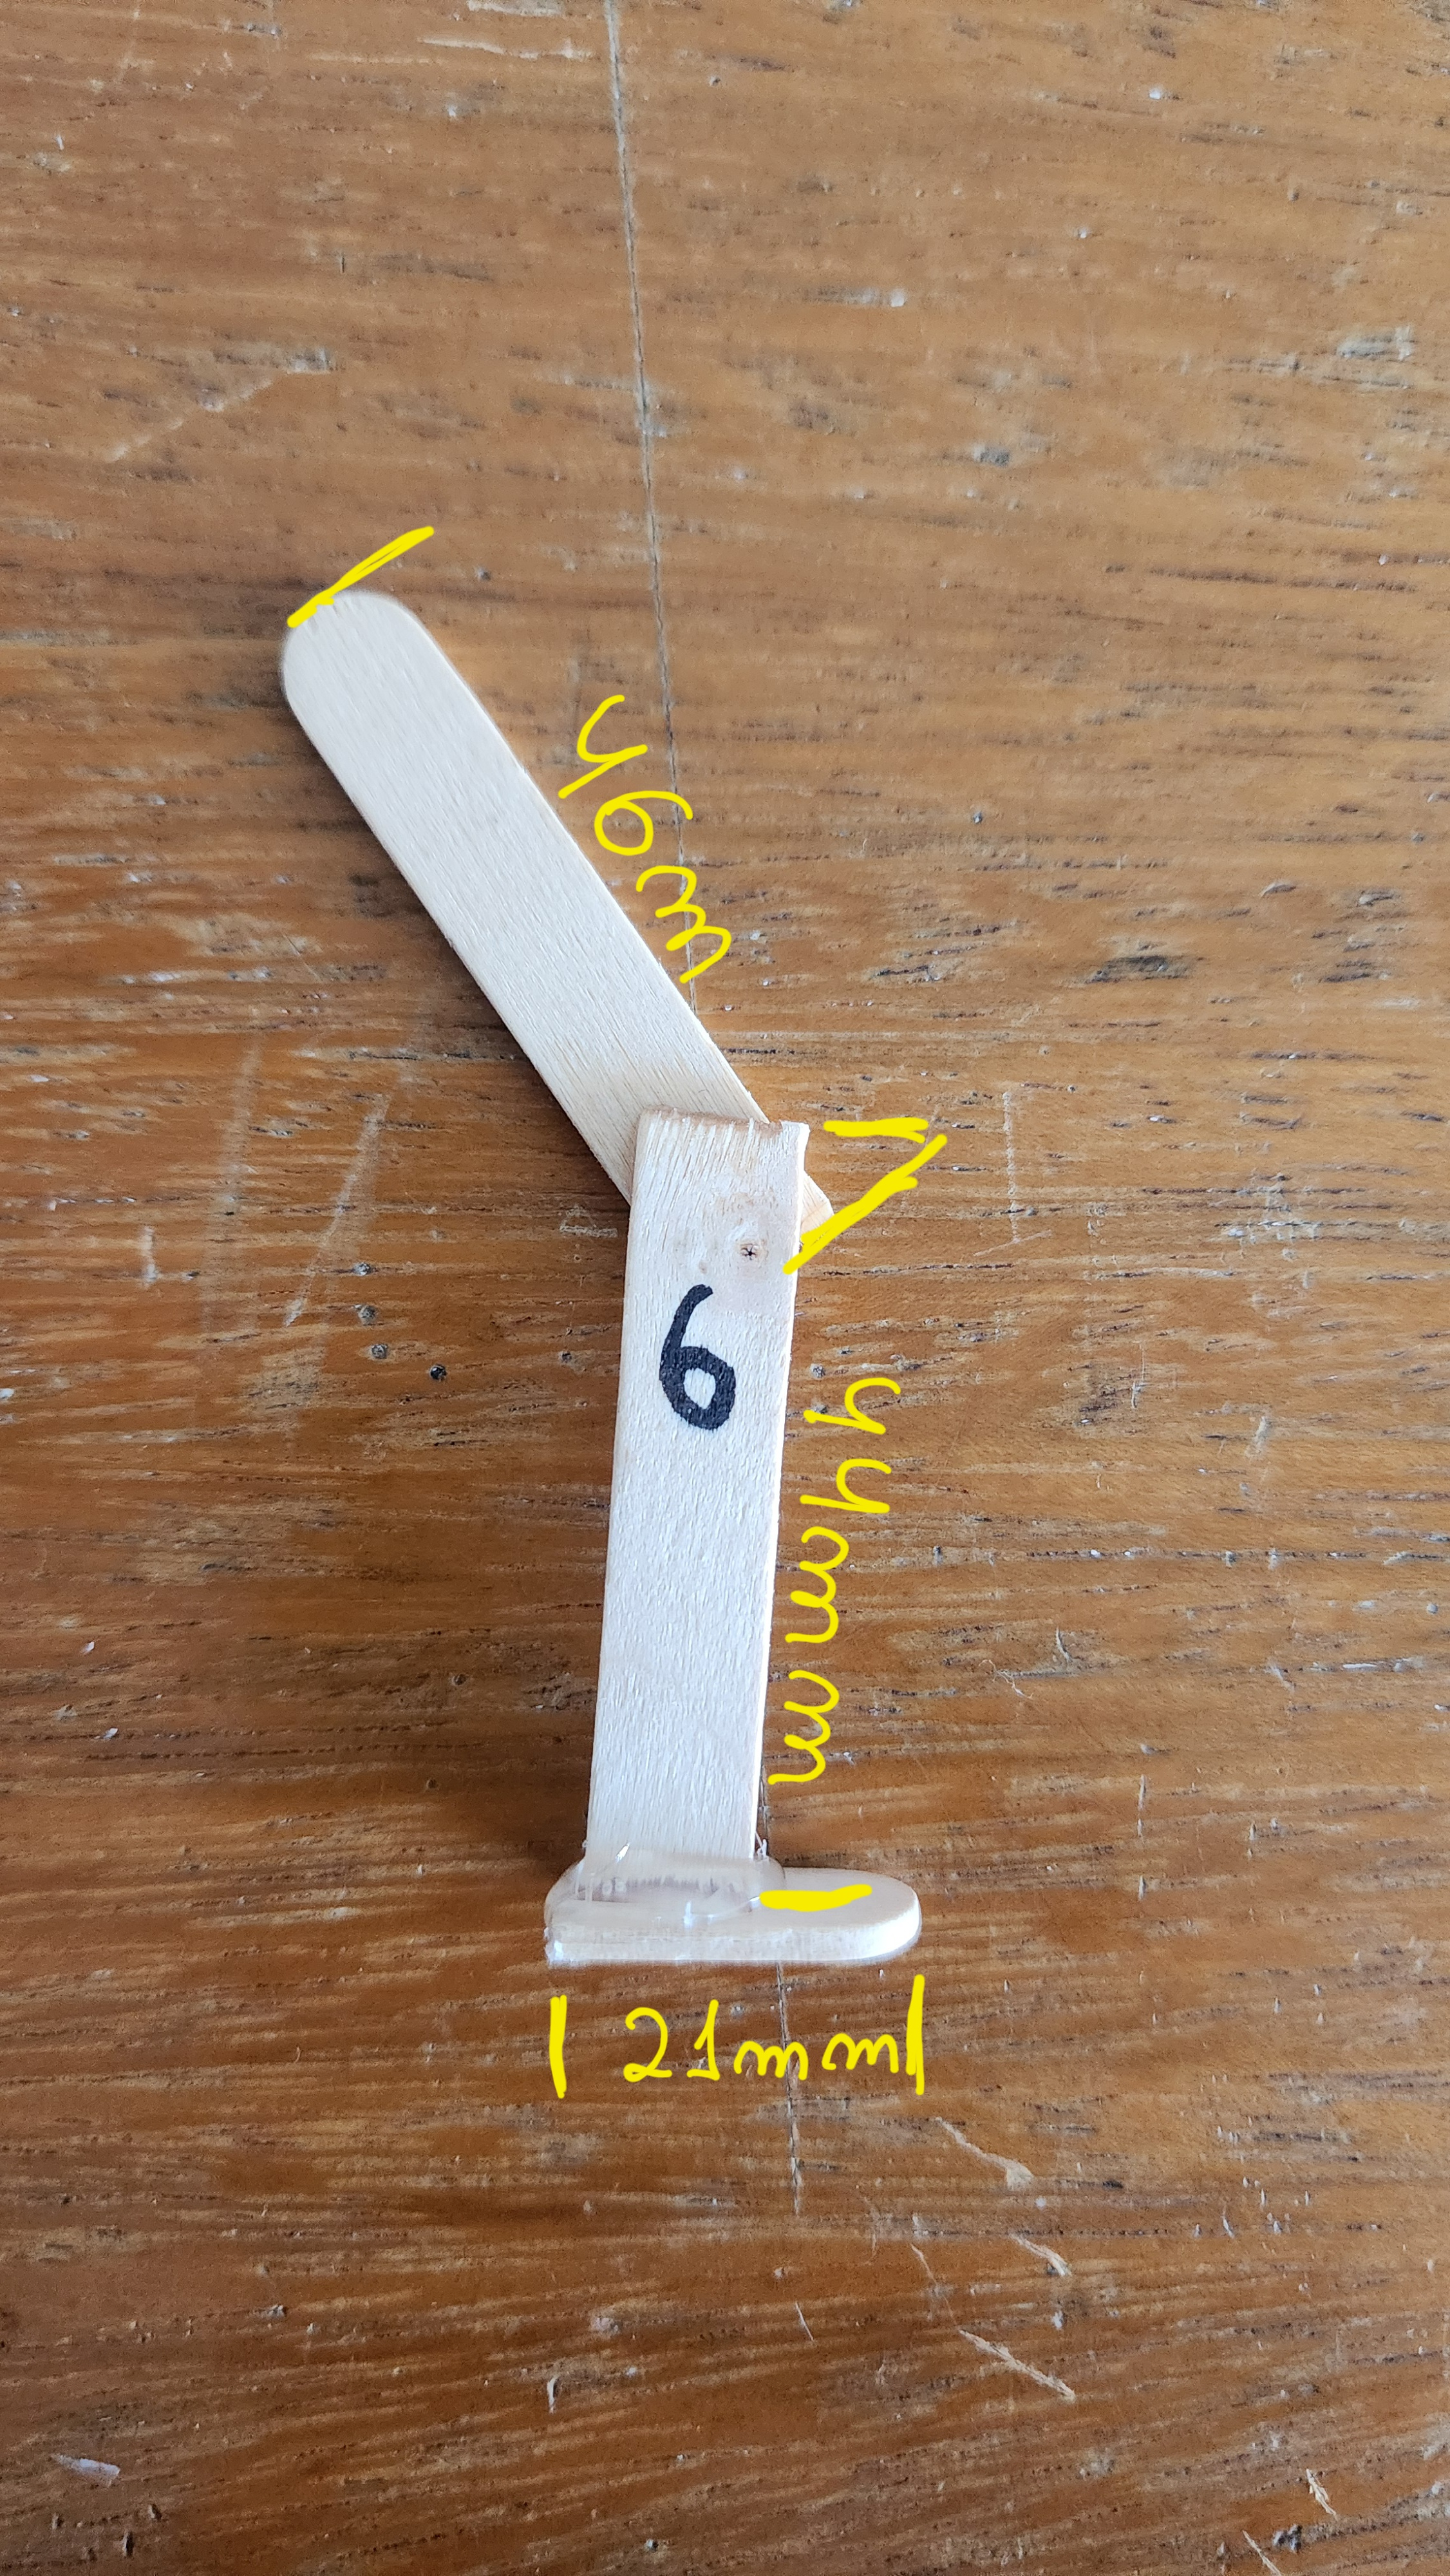
\includegraphics[width=10cm]{foto_parte5.jpg}
\caption{\label{fig:parte5}- Detalhe e dimensões da Perna (visão lateral).}
\end{center}
\end{figure}

\begin{figure}[H]
\begin{center}
 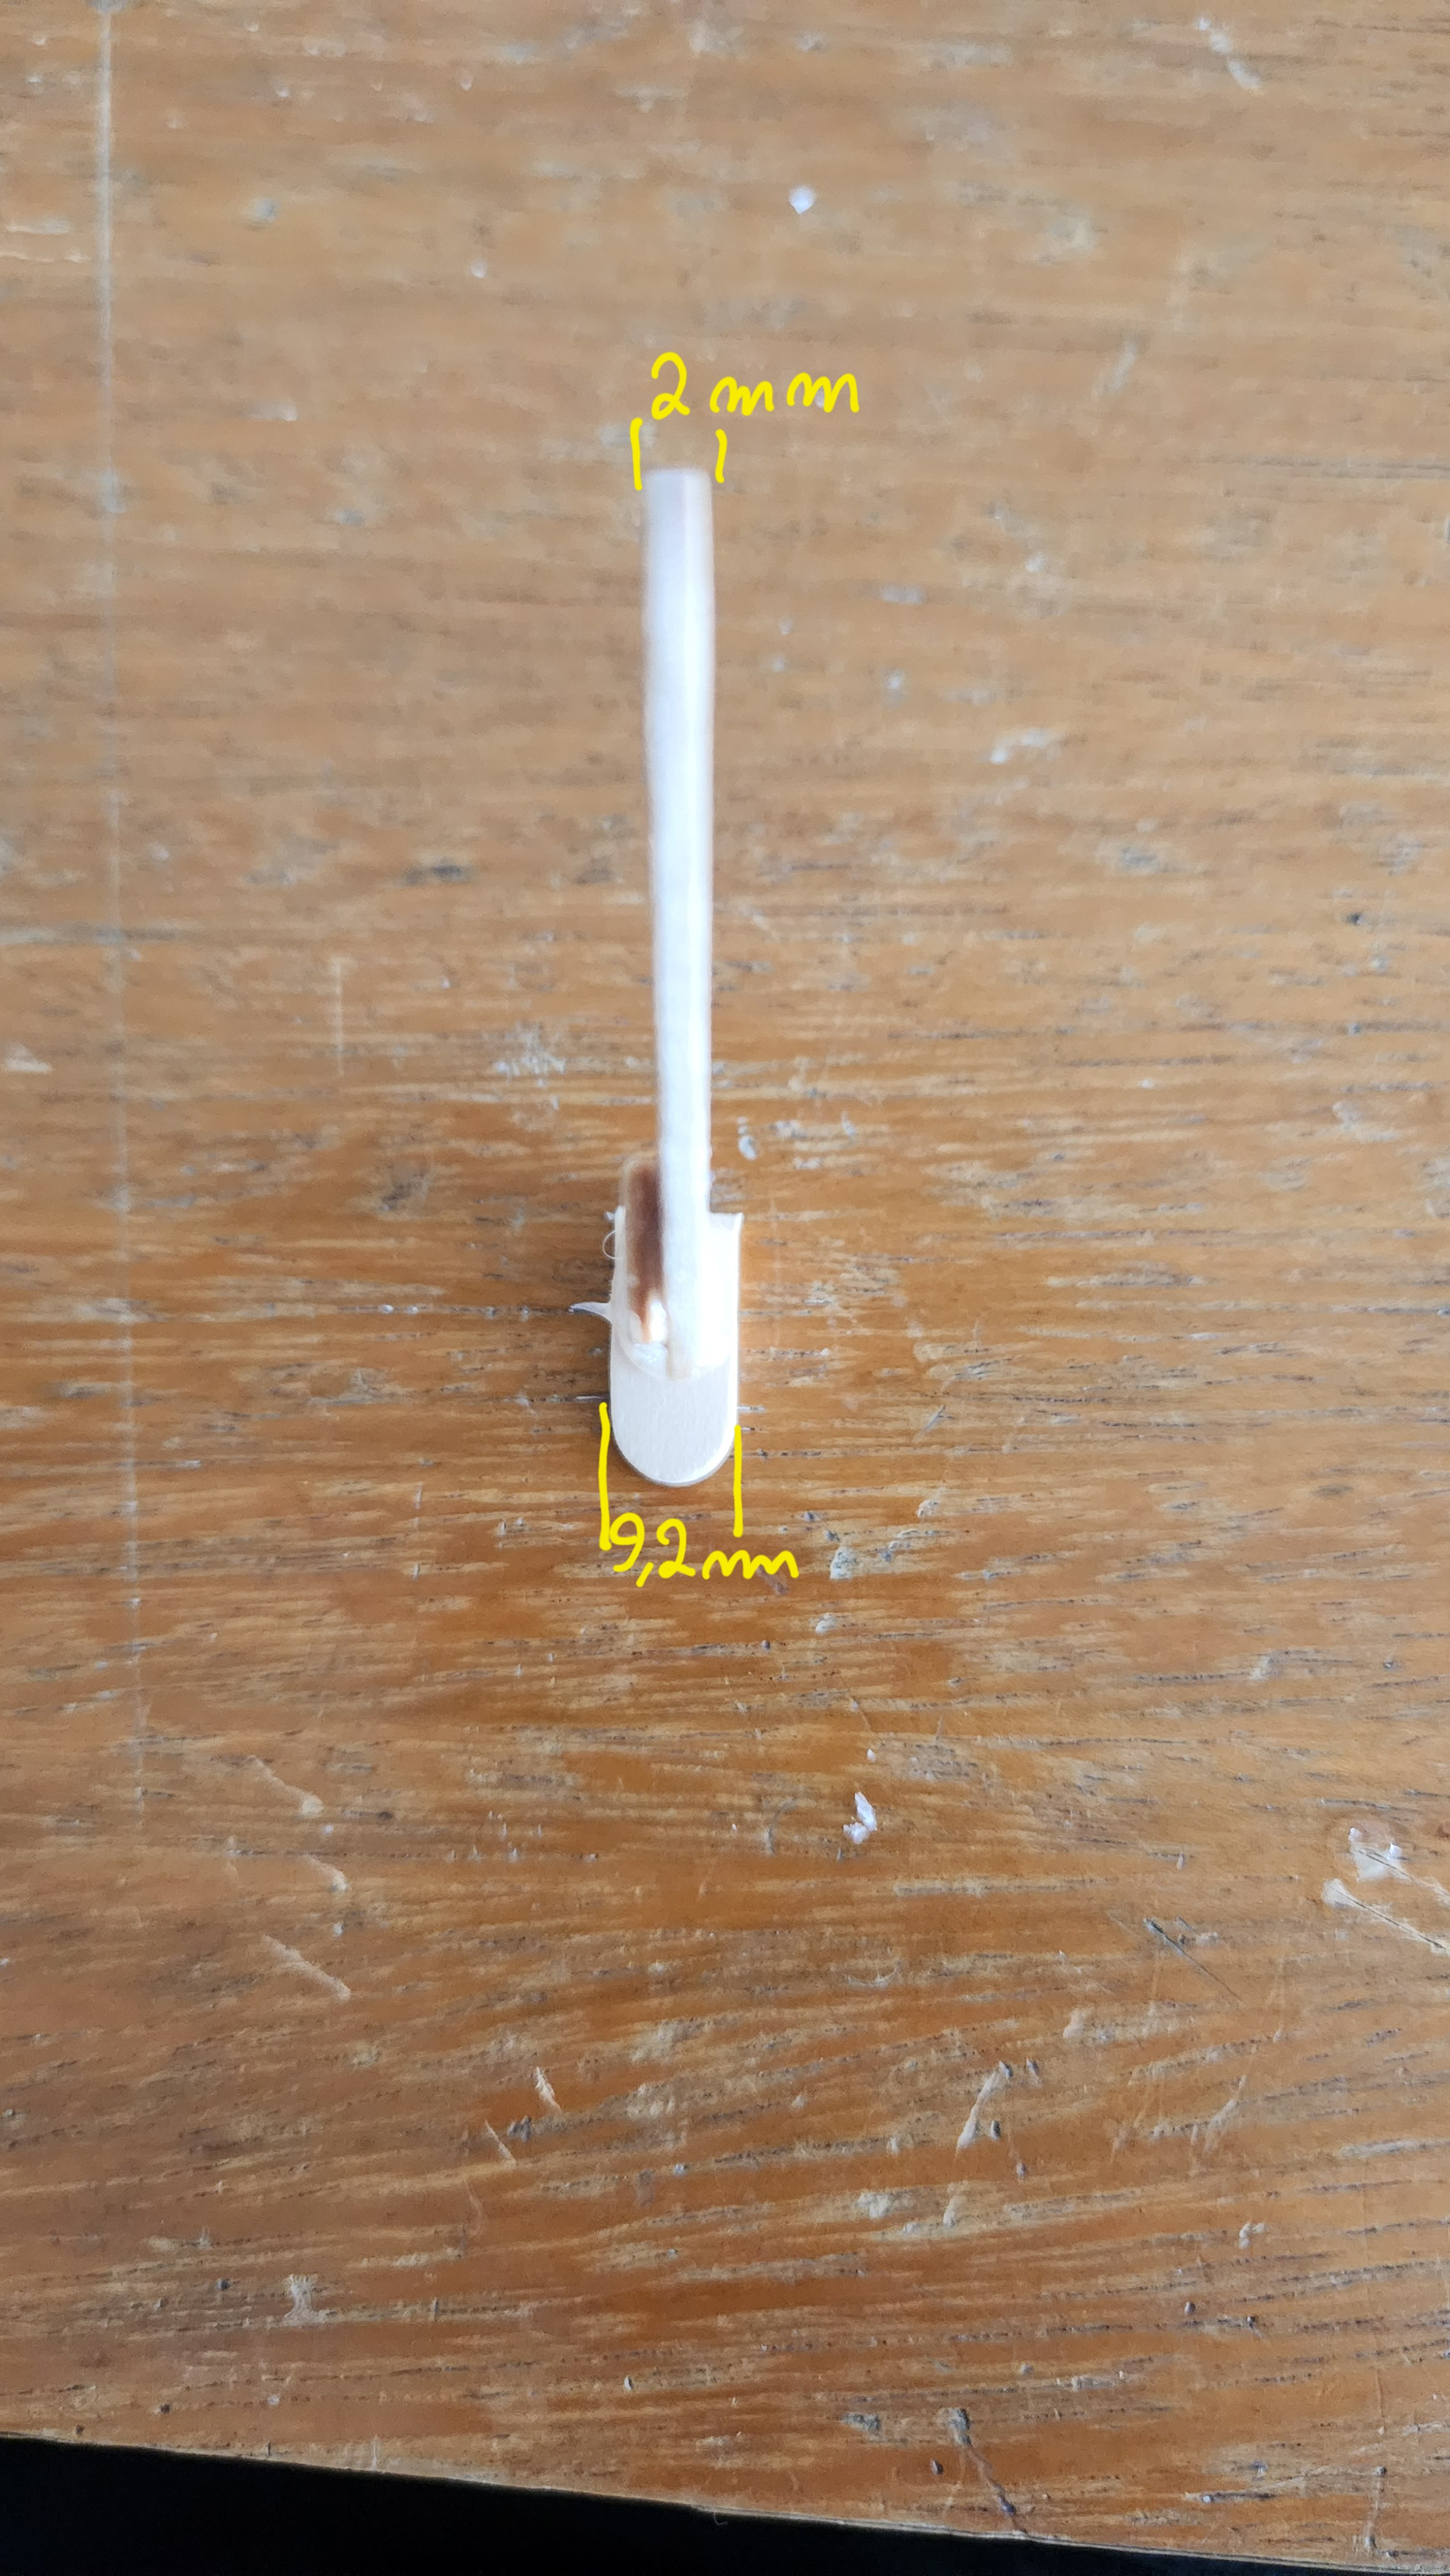
\includegraphics[width=10cm]{foto_parte6.jpg}
\caption{\label{fig:parte6}- Detalhe e dimensões da Perna (visão frontal).}
\end{center}
\end{figure}

\subsection{Medição dos Ângulos}

Os ângulos entre os segmentos do braço e da perna foram obtidos das fotografias das peças apoiadas sobre a bancada e fotografadas de cima. Em cada fotografia, os pixels de cada segmento foram isolados por um limiar de cor e de saturação, e uma reta foi ajustada a cada um por decomposição em valores singulares; o ângulo entre as direções das retas é o desvio entre os segmentos. Na perna, a junta entre as hastes resultou em um ângulo interno de 138,8$^\circ$. No braço, a medição com transferidor resultou em 130$^\circ$ e o ajuste de retas na fotografia da peça em 140,8$^\circ$ (desvio de 39,2$^\circ$); adotou-se o ângulo interno de 150$^\circ$, para o qual o avanço horizontal do segmento inclinado (23,3 mm) é praticamente igual à distância de 22 mm do plano do braço ao plano de simetria, de modo que as mãos se encontram sobre a corda, como se observa na vista frontal do protótipo. Na perna, as distâncias do calcanhar (7,0 mm) e do dedão (14,0 mm) ao eixo da haste foram obtidas da mesma fotografia, com o comprimento do pé (21 mm) como escala.

\subsection{Dimensões das Peças}

A \ref{tab:geometria} reúne as dimensões usadas no modelo. Todas as peças de madeira têm seção do palito de picolé (9,2 mm $\times$ 2,0 mm).

\begin{table}[H]
\centering
\caption{\label{tab:geometria}- Dimensões das peças utilizadas no modelo.}
\vspace*{.1cm}
\small
\begin{tabular}{|l|p{9.2cm}|}
\hline
\textbf{Peça} & \textbf{Dimensões} \\
\hline
Braço & segmentos de 90,0; 46,6 e 16,8 mm; ângulo interno da junta de 150$^\circ$ e do gancho de 70$^\circ$ \\
\hline
Perna & hastes de 44,0 e 46,0 mm; pé de 21,0 mm (calcanhar de 7,0 mm e dedão de 14,0 mm em relação ao eixo da haste); ângulo interno do joelho de 138,8$^\circ$ \\
\hline
Ombro & camada inferior de 19,2 mm e duas camadas de 13,0 mm, com 9,2 mm de largura e 5,5 mm de altura total; furo de 5,0 mm; pino de 3,5 mm de diâmetro e 29,1 mm de altura total; raio da manivela de 9,0 mm \\
\hline
Quadril & haste de 3,5 mm de diâmetro e 84,2 mm de comprimento \\
\hline
Motor com caixa de redução & caixa de 22,5 $\times$ 31,8 $\times$ 18,8 mm; comprimento total de 64,2 mm; corpo do motor de 15,0 $\times$ 30,0 $\times$ 22,5 mm (15,0 mm estimado); eixo duplo de 5,4 mm de diâmetro e 36,8 mm no total \\
\hline
Bateria & 33,55 $\times$ 13,9 $\times$ 67,7 mm \\
\hline
\end{tabular}
\end{table}

\subsection{Parâmetros Adotados}

Alguns parâmetros não foram medidos e foram adotados por hipótese; eles são listados na \ref{tab:adotados} e devem ser substituídos por valores medidos quando disponíveis.

\begin{table}[H]
\centering
\caption{\label{tab:adotados}- Parâmetros adotados por hipótese.}
\vspace*{.1cm}
\small
\begin{tabular}{|p{5.6cm}|p{4.2cm}|p{4.5cm}|}
\hline
\textbf{Parâmetro} & \textbf{Valor} & \textbf{Observação} \\
\hline
Repartição da massa do motor & 40\,\% na caixa e 60\,\% no motor & motor mais denso \\
\hline
Largura do corpo do motor & 15,0 mm & não consta do desenho \\
\hline
Massa dos palitos compostos & proporcional ao comprimento & seção e material iguais \\
\hline
Furo da perna no quadril & 4,6 mm da extremidade & metade da largura do palito \\
\hline
Posição da bateria & atrás da caixa, centrada & estimada da fotografia \\
\hline
Altura da junta do braço & 24 mm acima do eixo do motor & lida na fotografia frontal \\
\hline
Rotação do motor & 30 rpm no eixo de saída & valor suposto \\
\hline
Amortecimento & $c_{ch}=10^{-4}$ e $c_p=5\cdot10^{-5}$ N$\cdot$m$\cdot$s/rad & valores supostos \\
\hline
\end{tabular}
\end{table}
